\documentclass[12pt]{report}

\usepackage{amsmath}
\usepackage{graphicx}
\usepackage{tabularx}
\usepackage{natbib}
\usepackage{todonotes}
\usepackage{amssymb}
\usepackage{amsfonts}
\usepackage{amsthm}
\usepackage{mdframed}
\usepackage{float}
\usepackage[labelfont=bf]{caption}
\usepackage{soul}
\usepackage{dsfont}
\usepackage{mathtools}
\usepackage{algpseudocode, algorithm}


% To do commands
\newcommand{\slava}[1]{\todo[color=blue!40]{#1}}
\newcommand{\trish}[1]{\textrm{\hl{#1}}}

\linespread{1.6}

\title{Master's Proposal}
\author{Slava Nikitin}
\date{\today}

\begin{document}
\maketitle

\tableofcontents

\listoftodos
\begin{itemize}
\item Add a table density definitions used in the proposal
	  MAYBE
\item Graphs for models
	  MAYBE FOR FINAL COPY
\end{itemize}

%%%%%%%%%%%%%%%%%%%%%%%%%%%%%%%%%%%%%%%%%%%%%%%%
\chapter{Introduction}
%%%%%%%%%%%%%%%%%%%%%%%%%%%%%%%%%%%%%%%%%%%%%%%%

Under the same environmental conditions humans, and other phylogenetically younger animals, show a limited number of alternative behaviors. Variability of behavior suggests that evolution of complex perceptual and cognitive functions presents animals with choices for any given situation. Given that behavior is organized successfully in light of choices, their nervous systems must have a mechanism for transforming competing choices into a decision. Thus, understanding how the brain organizes behavior of complex animals can be advanced by understanding decision mechanisms it empoys.

Laboratory investigations of decision-making involving humans span a wide range of decision situations. Humans can be asked to make complex, multi-step decisions involved in selecting among health care policies \citep{PetHar2014}, gambles \citep{TveKah1981}, competitive strategies \citep{Cam2003}, and to make simple one-shot decisions based on a single dimension of a stimulus such as presence of a visual pattern \citep{Smi1995}, relative brightness of stimuli \citep{RatRou1998}, or motion direction \citep{RatMck2008}. In this thesis, I will concentrate on simple one-step decisions among two alternatives because resulting behavioral data can be obtained under rigorous control \citep{ZanTow2013}, the decision process is more amanable to mathematical modeling \citep{Coo1983,LewFar2010}, and the uncovered principles may generalize to all forms of decisions \citep{ShaKia2013}.

An example of laboratory tasks I concentrate on is a lexical decision task \citep{Wag2009}. On each trial, a participant is shown a string of letters, and asked to quickly and accurately decide whether it is a word or not by pressing one of two buttons on a response box. Thus, the design of an experiment couples participant's decision with a simple movement \citep{ZanTow2013}, and enables easy collection of responses, response times and physiological measures that can provide substantial clues about the simple decision mechanism \citep{Luc1986,ShaKia2013,MulMaa2014}.

The data bearing on psychological theory of simple decisions comes from both neural and behavioral studies. On one hand, the key findings from neural studies involve growth and decay shapes of firing rate functions of neurons interpreted as implementing competing decisions \citep{GolSha2007}. On the other hand, behavioral data constributes response rates and response time distributions, which have had the most effect on theory so far and will be the focus of the thesis \citep{Sto1960,Edw1965,Vic1979, TowAsh1983,Luc1986,ShaNew1996,RatRou1998,SmiRat2004,Bog2007,MulMaa2014}. The primary features of behavioral data include positively skewed response time distributions, asymmetries between correct and error means, speed-accuracy trade off and sequential relations between consecutive responses and response times \citep{CraPer2010,Rat2014}. 

The currently dominant theoretical understanding of simple one-stage decisions is based on analogy with sequential sampling of data from statistics \citep{WalWol1948, Sto1960,Vic1979, BogBro2006}. One version of psychological theory consistent with sequential sampling postulates that on every trial participant's brain forms a variable representation of the decision-relevant stimulus feature. In order to make a decision, participants have a mechanism to sample noisy signals from the representation and accumulate them into separate representations standing for competing choices. A decision is formed once one of the choice representations, called evidence integrators, reaches a preset and stable threshold of evidence. Associated movement execution follows depending on which evidence integrator reached the threshold first. 

There are several competing models that implement sequential sampling idea in a mathematical formalism  \citep{Sto1960,Pik1973,Rat1978,UshMcc2001,BroHea2008}. Assumptions of the models provide a precise description of how various parameters of processing combine to form simple decisions, parameters that are supposedly capturing higher-level properties of a task-evoked neural network \citep{GolSha2007,CasHea2014,MulMaa2014,ColBas2014}. The models highlight time to encode evidence, rate of evidence uptake, evidence threshold, initial evidence and time to execute a motor response as important processing parameters in explaining patterns of behavioral data, but make different assumptions about how these parameters combine to generate choice behavior. 

One way to categorize all the models is based on three types of assumptions that they make. The first kind of assumptions describe the number, interactions and dynamics of evidence integrators during a trial, potentially expressed as a system of stochastic processes \citep{Smi2000}. The second kind makes assumptions about other stages of processing involved in a trial, such as encoding of stimulus features and motion response, which frequently amounts to assigning an overall time constant that describes their duration \citep{RatSmi2004}. Lastly, simple decision models incorporate distributional assumptions that describe how parameters vary across trials to capture variability in the processing system \citep{RatSmi2004, JonDzh2014}. 

Mathematical assumptions of the competing models make different theoretical claims about processing, and testable predictions about responses and response time distributions can be deduced from the assumptions \citep{Vic1979,Coo1983,Luc1986}. A set of models, widely used for providing process-based interpretation of behavior \citep{RatMck2008,DonBro2011,HeaHay2012} models have been developed that all account, with high accuracy, for a large number of patterns in behavioral data including response time distributions, accuracy, and relations between response times and accuracy, across a variety of manipulations and paradigms \citep{UshMcc2001,RatTue2002,BroHea2008}. The problems with these models are that they mimic each other statistically with common sample sizes while making different theoretical claims \citep{ZanCol2000,RatSmi2004,DonBro2011}, and they do not yet account for the whole pattern of behavioral data.

One of the ways to push undestanding of a simple decision process forward is to incorporate additional theoretical principles into promising models and attempt to account for unexplained data patterns. Looking at the history of the sequential sampling field, one of the largest differences between currently popular models and their predecessors is addition of assumptions about variability of parameters across trials \citep{Lam1968,Vic1979,RatSmi2004}. Variability assumptions express the idea that processing is not static across trials within a condition. Starting evidence may include evidence remaining from the previous trial or movement time may be faster if the same stimulus repeats. Expressed in terms of probability distributions, variability enabled to account for additional data involving asymmetries in relations between speed and accuracy of processing, which the old models missed \citep{Luc1986, RatSmi2004}. 

While some gains in understanding have already been made from incorporating trial-to-trial variability in parameters into models, I suggest that further gains can be made by better characterizing this sort of variability. Consider that currently popular models differ in assuming what parameters vary and what their distributional forms are \citep{JonDzh2014}, but they all commit to two questionable claims: on each trial a parameter is set to a value independent of the previous trials and all parameters are mutually independent \citep{UshMcc2001,RatTue2002,BroHea2008}.

The first assumption is challenged by the always present auto-correlation in response times and responses \citep{PerVan2002, JonCur2013}. The behavior suggests that, say, evidence threshold of a participant on one trial depends on the threshold value on the previous several trials \citep{VanMal2004}. One line of recent model development incorporated the principle of auto-correlated parameters through additional processes including learning of stimulus probabilities, error-correction and residual evidence \citep{ChoNys2002,WagFar2004,BroMar2008,GaoWon2009,GolWon2012}. Depending on the model, starting evidence, rate of evidence uptake and evidence thresholds were functions of values on previous trials and parameters of additional processes. Such modifications enabled models to predict a variety of sequential effects and improve understanding of decision process dynamics.

However, the other questionable assumption, the issue of mutual independence of processing parameters, has not been examined. An alternative to independence is that processing parameters vary in systematic ways from trial to trial. Several sources of evidence provide support for statistical dependence among parameters.

One form of evidence comes from model-based analyses of response time distributions under block-wise manipulation of speed-accuracy instructions. Using a couple of prominent sequential sampling models, researchers showed that the best explanation of accuracy emphasis is based on simultaneous rise in the rate of evidence accumulation and evidence threshold \citep{VanTue2007,VanTue2011,RaeHea2014}, and sometimes also increase in non-decision time \citep{VosRot2004,ZhaRow2014}. In further support of change in non-decision time, a purely empirical study, using measurements of lateralized readiness potential with electroenchepolagraph, demonstrated that under speed instructions the time interval between onset of motor processing and motor response decreases \citep{RinOsm2004}. Both kinds of studies suggest that a control process that sets a speed-accuracy regime, as manipulated by instructions, can modulate activity in two or more parts of a task-evoked neural network and its affects are picked up by the models' parameters  \citep{Wan2008,HarSch2011,TurFor2013,ColBas2014}.

Another block-wise manipulation indicating systematic tradeoffs among parameters is due to practice. Using a sequential sampling model to analyze 10,000 trials of the lexical decision task, researchers found a coordinated adjustment of processing parameters with practice \citep{DutVan2009}. The nondecision time decreased, rate of evidence uptake increased, evidence threshold decreased and initial evidence became less biased with practice. In a similar model-based study, but based on a motion discrimination task, participants showed decrease in the evidence threshold and increase in the rate of evidence uptake over 4032 trials \citep{ZhaRow2014}. Overall, practice effects are also consistent with a principle that decision and non-decision parameters change in a dependent manner. 

On a trial-by-trial level, the phenomenon of post-error slowing also suggests dependencies among parameters as a feature of sequential decision-making \citep{VanMal2004}. Post-error slowing refers to a phenomenon when a participant makes a mistake, response time on the next trial slows down. Explanations of this phenomenon have usually envoked only an increase in evidence threshold, but a model-based analysis showed that rate of evidence uptake, evidence threshold and nondecision time may all be affected \citep{DutFor2013}. \citet{DutFor2013} examined old and young adults with lexical decision and motion discrimination tasks. Old adults showed increase in evidence threshold, decrease in rate of evidence uptake and increase in non-decision time across both tasks. Young adults showed increase in non-decision time in the motion discrimination task, but in the lexical decision task they increased evidence thresholds and increased non-decision time. 

Another sequential effect that is consistent with dependent parameters is based on effects of prior stimuli on response times. \citet{GolWon2012} gathered behavioral data for a task requiring discrimination between upper and lower case of letter "o". They analyzed mean response times, separated by correct and error response, on the second trial of two-stimulus sequences consisting of all possible combinations of repetitions and alternations. Conditioned on stimulus sequence, participants showed trade-offs between correct and error response times: faster response time on error trials would correspond to slower response times on correct trials, or vice versa. Model with trial-varying initial evidence captures the qualitative pattern, but systematically misses response times for error trials. Given the mechanics of sequential sampling models, the misses may be due to not accounting for adjustments in thresholds or rate of information uptake that happen simultaneously with initial evidence.

An account of sequential effects based on simultaneous adjustment in parameters has been proposed by \citet{RatZan1999}. Subjects were given a numerocity task where clusters of asterisks need to be discriminated as large or small. Some subjects showed elevated probabilities and speed when repeating the previous response rather than altering the response. Explanation of both the response probability and response time was successful only when initial evidence and rate of evidence of uptake were allowed to adjust simultaneously. 

Finally, on a more speculative note, one possible basis of parameter correlations is suggested by studies of control processes, such as task instruction processing, task representation, error monitoring, selective attention, that are found to frequently (on the order of seconds) modulate task-evoked brain network in line with task demands and statistical structure of stimuli \citep{MozKin2007,JonKin2009,ColFra2013}. The neural basis of control processes has been generally assigned to prefrontal cortex and basal ganglia \citep{SchAar2010}, regions which have two-way projections to almost all the other structures in the limbic system and neocortex \citep{MilCoh2001,CalPic2014}. Hence, current understanding of neural architecture of the control processes provides an opportunity for simultaneous modulation of activity in all components of a task-evoked network supporting particular speeded decisions. 

Behavioral and neural data presented above suggests, without being conclusive, that there may be correlations between processing parameters underlying simple choice behavior. While other interpretations are possible, I propose to quantify evidence for a simple and falsifiable principle of processing dynamics underlying visually-guided choice behavior: from trial to trial, and across conditions, psychological parameters identified by sequential sampling models vary systematically in a dependent manner. The suggested ``dependence principle'' is in qualitative contrast with the usually assumed independence of processing parameters \citep{RatSmi2004}. 

Given the sharp contrast between the proposed and the conventional principle, the goals motivating the proposed thesis are to generalize one of the currently popular sequential sampling models of decision and study its relation to a model with independent parameters. The proposed approach involves adding a correlation structure, that in addition to location and scale, can describe correlations between parameters without making a theoretical claim as to how correlations arise. Using a generalized model several questions can be posed and answered: Do models with and without dependencies lead to different time courses of the decision process? Are behavioral predictions distinguishable between them?  What can we extract from data about parameter correlations? How much does predictive accuracy increase when adding a correlation structure? In the end, addressing these questions through theoretical and empirical comparisons of the standard version and a generalized version of a sequential sampling model can give a better insight into processing underlying choice behavior.

In the rest of the introduction chapter, I will lay out reasons for taking formal modeling approach to test the dependence principle and elaborate the structure of experiments generating behavioral data. As an example of a typical experiment, I will present a benchmark dataset, and important response time and accuracy features that will form the focus of comparisons between models. After, I will present standard sequential sampling framework and then introduce a method of constructing multivariate distributions that will be useful for developing a generalized model of decision making. Finally, I will present a statistical framework grounded in Bayesian theory that will be used to estimate the correlation structure and compare predictive accuracy of proposed models.

%%%%%%%%%%%%%%%%%%%%%%%%%%%%%%%%%%%%%%%%%%%%%%%%%%%
\section{Formal Modeling Approach}
%%%%%%%%%%%%%%%%%%%%%%%%%%%%%%%%%%%%%%%%%%%%%%%%%%%

Psychology has as one of its chief aims understanding of the cognitive
architecture that generates the rich repertoire of human behavior and is
sensitive to many environmental variables \citep{AndBot2004,And2007}. More
specifically, a psychologist wants to learn about the number, temporal
arrangement, properties and interactions of elementary
processes that organize behavior. A fundamental obstacle to satisfying psychologist's aspirations is
that cognition is not directly observable. For instance, we can observe a person engage in different behaviors under the same conditions, but the process of action selection is latent. Even if we had the whole wiring diagram of the person's brain and spiking patterns under a variety of situations, it still would not be obvious where, how and when action selection takes place \citep{Bro2014}. So, how to go about it?

Concentrating on behavioral methodology, the study of human cognition can be considered as an instance of a black box
problem \citep{Lju1999, Lju2010}. Working on a black box problem, a
researcher only has direct information about the system's input and
output, but lacks direct access to internal processes transforming inputs
into outputs. The original problem can then be formulated as how to understand internal processes from
known combinations of inputs and outputs, or in psychological terms, how to uncover the human
cognitive architecture from information about overt behavior taking place
in some environment.

A powerful approach to providing an approximate solution to the black box problem
is construction of competing mathematical models that can be
tested against data using statistical methods
\citep{Lju1999,Lju2010,CasBer2002,GelCar2013}. Each model would represent a mechanistic account of how inputs are transformed into outputs. A model that best balances
parsimony, fit to known empirical regularities and interpretability can be taken
as a formal instantiation of the best theoretical principles characterizing internal processes and provide further guidance in experimental work. This approach fits well with psychological
research because it is often easy to come up with several, categorically
different conjectures about underlying cognitive processes
\citep{Vic1979,TowAsh1983} and there is plenty of data to constrain them \citep{Luc1986}.

The primary benefit of developing mathematical models rather than verbal descriptions is that they force coherency on theoretical assumptions, enable deriving exact conclusions from assumptions and improve falsifiability of proposed principles through quantitative statistical testing
\citep{Coo1983,BusDie2010,LewFar2010,LeeWag2014}. For instance, a model of memory processes that can
predict a power relation between time and memory retention is easier to falsify than a verbal account that only makes ordinal predictions \citep{CavMyu2013}. Ultimately, the promise of mathematical models is to bring psychology closer and faster to sensible theoretical principles that characterize elementary processes and how they evolve over time, under different
experimental conditions for different individuals.

Before presenting an example of the formal modeling framework, I will describe notation used for the rest of the thesis. I will use lower-case non-bolded symbols for scalars, lower-case bolded symbols for column vectors, and upper-case bolded symbols for matrices. I will discriminate between random variables and their realized values by qualifying my statements when necessary, but otherwise their case will reflect their mathematical nature (i.e. scalar or vector), as for other symbols. Observables, response variables or covariates, will be represented with Roman letters while parameters will be represented with Greek letters.

A formal relationship between response variables $\mathbf{y} \in \mathcal{Y} \subseteq \mathbb{R}^k$, covariates $\mathbf{x} \in \mathcal{X} \subseteq \mathbb{R}^l$ and parameters $\mathbf{\theta} \in \Theta\ \subseteq \mathbb{R}^m$, will be stated as a parametric statistical model $M = \{F(\mathbf{y} \mid \boldsymbol{x}, \boldsymbol{\theta})\}$, where $F$ is a probability distribution function. In words, a parametric model is a collection of probability distributions indexed by a finite-dimensional parameter that provides a full description of variability in $\mathbf{y}$. If a probability density (mass) function $f$ exists, then a model expression can be stated in terms of $f$. Also, covariates may not always be present, so $\mathbf{x}$ may be dropped. Lastly, a short-hand notation $\mathbf{y} \sim F(\mathbf{y} \mid \boldsymbol{\theta})$ may be used, where $\sim$ stands for ``distributed as''.

As an example, consider a random vector $\mathbf{y} = (y_1, y_2, \ldots, y_n)^T$, where T is a transpose operator. If we assume that $\mathbf{y} \in \mathbb{R}^n$ varies according to a multivariate normal probability density $f$, parameterized with a vector $\boldsymbol{\mu} \in \mathbb{R}^n$ and a positive definite matrix $\boldsymbol{\Sigma} \in \mathbb{R}^{n\times n}$, then the parametric model of $\mathbf{y}$ is a collection of probability densities  
\begin{equation}
M = \left\{f(\mathbf{y} \mid \mu, \sigma^2) = \det(\sqrt{2\pi}\boldsymbol{\Sigma})^{-1} \exp\left(-\frac{1}{2}(\mathbf{y} - \boldsymbol{\mu})^T\boldsymbol{\Sigma}(\mathbf{y}-\boldsymbol{\mu})\right)\right\}, 
\end{equation}
where $\det(\cdot)$ is a determinant operator.

With notation fixed, I will briefly present the formalism of the standard signal detection theory as an example of approach taken to testing dependencies among parameters during simple choice behavior \citep{MacCre2004}. The original phenomenon motivating development
of signal detection models was human ability to make decisions with
distorted sensory stimuli. This phenomenon can be studied experimentally
using a computerized task. For example, during the auditory signal
detection task an observer is presented with a sequence of stimuli drawn
either from a \textit{Signal} distribution representing a tone combined with
white noise, or a \textit{Noise} distribution representing white noise. On each
trial, an observer has to respond ``Yes'' if he or she decides the
stimulus belongs to the \textit{Signal} distribution and ``No'' otherwise. Under
these conditions, a researcher knows which class each presented stimulus
belongs to and observes a sequences of responses, typically summarized as
hit rate (proportion of true positive responses) and false alarm
rate (proportion of false positive responses). The psychological problem is to
characterize cognitive processes involved in transforming stimulus
information into responses from the generated data.

Signal detection models are statistical models that decompose hit and false alarm rates into cognitively interpretable parameters characterizing stimulus representation and decision process without specifying mechanistic details
\citep{MacCre2004,LeeWag2014}. The basic idea is that behavior in a
signal detection task can be explained by a theory that
proposes the following principles:
\begin{enumerate}
\item Presentation of a stimulus causes observer to form a  representation of the stimulus ``strength.''  
\item An observer is able to establish a decision threshold to which this perceived strength can be compared.  
\item If the perceived strength is greater than this threshold then the 
      observer responds ``Yes,'' otherwise he or she responds ``No.''  
\item The perceived strength varies from trial to trial such that its statistical structure (mean and 
      variance) is determined by the class of the presented stimulus, where the strengths of Noise stimuli tend to be perceived as being below 
      the threshold and the strengths of Signal stimuli tend to be perceived 
      as being above.  
\end{enumerate} 

Formalization of these principles can be done using language of probability theory \citep{CasBer2002}. Let a random variable $c \in \{0, 1\}$ represent a stimulus
randomly drawn either from the \textit{Noise} class ($c = 0$) or
the \textit{Signal} class ($c = 1$). The probability mass function of
$c$ is determined by the experimenter. In response to the sampled
stimulus, an internal representation of strength value, represented
by a random variable $x \in \mathbb{R}$, is generated. We commonly
assume that $x$ conditioned on the stimulus class is normally
distributed with class-specific mean $\mu_i \in \mathbb{R}$ and variance $\sigma_i^2 > 0$ parameters, so that
%
\begin{align}
x \mid c = 1 \sim \mathcal{N}(\mu_s, \sigma_s^2) \text{and} \nonumber \\
x \mid c = 0 \sim \mathcal{N}(\mu_n, \sigma_n^2),
\end{align}
% 
where $\mid$ stands for ``conditioned on''.
Finally, let $\tau \in \mathbb{R}$ represent the position of a threshold on a strength dimension. Then a random variable
%
\begin{equation}
r = \left\{
	\begin{array}{l l}
     1 & \text{ if } x \geq \tau\\
     0 & \text{ if } x < \tau
     \end{array}\right.
\end{equation}
%
represents a ``Yes'' ($r=1$) or a ``No'' ($r=0$) response.

As written, this version of the model has five free
parameters ($\mu_n,\mu_s,\sigma_n,\sigma_s,\tau$), but
because normal distributions form a location-scale family, where the
mean and standard deviation are the location and scale parameters,
repectively, the means and standard deviations are identifiable only
relative to each other.  Therefore, we set $\mu_n = 0$ and $\sigma_n = 1$
without loss of generality. The other three parameters remain free,
and quantify representational and decision features of signal detection.

In actual analysis of behavioral data, it is common to use the derived parameter $d' = (\mu_s - \mu_n)/\sqrt{(\sigma_s^2 + \sigma_n^2) / 2} = \mu_s/\sqrt{\sigma_s^2 / 2}$, which is psychologically interpreted as quantifying how well
the encoding process separates \textit{Noise} from \textit{Signal} stimuli \citep{MacCre2004}. 
The threshold
$\tau$ represents the decision criterion
%
and the ratio of variances
$\sigma_n^2/\sigma_s^2 = 1/\sigma_s^2$ between \textit{Noise}
and \textit{Signal} distributions characterizes relative noise in
representations. These three parameters drive the predicted pattern of
responses.
    
To begin testing a specified cognitive model one needs to derive, or be
able to simulate, predictions for behavioral data. In the signal detection
case, the random mechanism specified above, and an additional assumption
that all responses during an experiment are mutually independent, allow for
an analytical derivation of a probability mass function parameterized by
the three free parameters.  The derived model for the number of hits
$y_h \in \{0, 1, \ldots, N_s\}$ and the number of false alarms $y_{fa} \in
\{0, 1, \ldots, N_n\}$ for a given participant presented with $N_s$
\textit{Signal} stimuli and $N_n$ \textit{Noise} stimuli is a product of two binomial probability mass
functions. The joint probability of $y_h$ and $y_n$, conditioned on parameters, is therefore
%
\begin{eqnarray}
\lefteqn{f(y_h, y_{fa} \mid p_h, p_{fa}, N_s, N_n) = }\nonumber \\
& & \binom{N_s}{y_h}p_h^{y_h}(1 - p_{h})^{N_s - y_h}
\binom{N_n}{y_{fa}}p_{fa}^{y_{fa}}(1 - p_{fa})^{N_n - y_{fa}},
\end{eqnarray}
%
with the probabilities $p_h$ and $p_{fa}$ being the probabilities
that $r=1$ conditioned on the stimulus class.  The hit and false alarm probabilities are in
turn functions of the representational and decisional parameters $\mu_s$, $\tau$ and $\sigma_s$, such that
%
\begin{align}
p_h = P\{r = 1 \mid c = 1\} = \Phi\left(\frac{\mu_s - \tau}{\sigma_s}\right) \text{and} \nonumber \\
p_{fa} = P\{r = 1 \mid c = 0\} = \Phi \left(-\tau\right),
\end{align}
where $\Phi(\:)$ is the standard normal distribution function and $P\{\cdot \mid \cdot\}$ is a conditional probability.
    
When a statistical model relating cognitive parameters to
data is specified for a given theory, one can use a rich body of
statistical methods to explore its predictions via simulations, to estimate
its free parameters from data, and to compare and select from
competing models of cognitive processing involved in a given task
\citep{Ber1997,CasBer2002,GelCar2013}. Connecting the signal detection
model to performance data enables a researcher to test underlying principles and make a range of
inferences about cognitive processes from behavior. For
instance, it is possible to test goodness of fit of a model with
$\sigma_s^2 = 1$ against a model where $\sigma_s^2$ is a free parameter to
determine the noise properties of the stimulus
representation. However, the range of possible inferences is limited, so
the specified model cannot say anything about (for example) formation and
adaptation of the representations to dynamic stimulus stream or motor processing. It would require a new model to address additional questions about processes involved in a signal
detection task.

The example of a standard signal detection model shows how experimental variables and behavioral data can be tied together in a formal model. With a formal model, theory of signal detection can be better tested and behavioral data can be interpreted in a psychologically interesting way. I intend to carry over these analytical advantages to my proposed studies of simple decision making. In the next section, I turn back to the problem of simple decision making and set the stage for later model development by elaborating on the structure of experimental tasks used to obtain behavioral data.

%%%%%%%%%%%%%%%%%%%%%%%%%%%%%%%%%%%%%%%%%%%%%%%%%%%%%
\section{Data-Generating Experimental Tasks}
\label{sec:tasks}
%%%%%%%%%%%%%%%%%%%%%%%%%%%%%%%%%%%%%%%%%%%%%%%%%%%%%
To obtain input-output data informative of processes underlying simple choice behavior, we need a laboratory task that requires processes of interest for above chance completion. I will consider simple choice behaviors to be a class of behaviors that rely on a single deliberation stage to form a discrete decision about an objectively determinable state of a noisy stimulus pattern during at most a two second window, starting with stimulus presentation and ending with movement registration. A large collection of tasks can evoke simple choice behaviors and can be classified in terms of five dimensions:
the sensory modality, the number of choices, the number of stimulus
attributes relevant to a decision, whether a
participant or an experimenter controls initiation of responses and response modality. For this thesis, I will concentrate
on participant-controlled two-choice tasks, where finger movements are driven by a single attribute of a visual stimulus. For short, I will call them two-choice tasks. 

Two-choice tasks have been the predominant kind for obtaining empirical regularities and developing theoretical models of simple decision making \citep{Lam1968,Vic1979,Luc1986,RatSmi2004,RatMck2008,Wag2009}.   
An example of a two-choice task is a numerosity task \citep{RatLov2012}. On a given trial, two clouds of points, consisting anywhere from a few dots to a hundred, are presented simultaneously on opposite sides of a computer screen. The relative number of points determines uncertainty about which cloud is more numerous. An observer has to make a decision, as accurately and as fast as she can, according to a rule that maps stimulus identity onto movements, such as ``press the button on a keyboard corresponding to a cloud with the larger number of points''. Once a movement is executed, it is easy to measure accuracy and response time using a computer.

Across trials of a two-choice task, several experimental variables are usually manipulated that have been found to produce recurrent empirical regularities in responses and response times \citep{Luc1986}. Continuing with the numerocity task, a researcher could vary relative number of points, instructions emphasizing either speed or accuracy, probability of the ``large'' cloud appearing on the left side and probability of transitions between ``large'' and ``small''. All of these manipulations tend to affect both accuracy and speed of responses, but in different ways, providing non-trivial constraints to test proposed models \citep{Vic1979,TowAsh1983}.

The combination of experimental variables and response variables generated by two-choice tasks make up the input-output data that can be used to learn about cognitive processing. In the next section, I will present a benchmark dataset generated by a brightness discrimination task that demonstrates the kind of patterns models need to satisfy.
    
%%%%%%%%%%%%%%%%%%%%%%%%%%%%%%%%%%%%%%%%%%%%%%%%%%
\section{Benchmark Behavioral Data}
%%%%%%%%%%%%%%%%%%%%%%%%%%%%%%%%%%%%%%%%%%%%%%%%%%
Two-choice tasks are simple, but under different experimental manipulations they generate many informative patterns in behavioral data. I will use the \citet{RatRou1998} brightness discrimination data as a source of behavioral data to test for dependencies among parameters. This dataset has become somewhat of a benchmark for testing new models because it has a large number of observations, and many of the recurrent accuracy and response time patterns \citep{VanTue2008,BroHea2008,VanTue2011,VerTue2014}.

\citet{RatRou1998} ran a brightness discrimination task with three participants. Each participant had one 35 minute practice session and ten 35 min experimental sessions. Each session consisted of eight blocks of 102 trials, for a total of 8160 trials. 

Each trial began with participants seeing a gray screen for 500 ms. After, an array of white and black pixels appeared at the center. Participants had to decide whether the array came from a ``high'' or ``low'' brightness distribution. They responded as soon as they could by pressing one of two buttons with the corresponding finger. Upon response, the stimulus would change back to the gray screen for a duration of 300 ms. During the final 300 ms, a feedback message was displayed indicating whether the decision is correct or not. Both responses and response times were recorded upon completion of a trial.

During each session, two experimental variables were manipulated. First, the
ratio of white to black pixels, representing stimulus difficulty, was manipulated across
trials. On each trial, a ratio was drawn from one of two symmetric, unimodal probability mass functions spanning over 33 levels of brightness and overlaping to ensure imperfect accuracy. Second,
every 204 trials instructions changed from directing participants either to
maximize speed or to maximize accuracy.

Overall, with a simplifying assumption that practice effects are negligible after the training session, the experiment generated a data matrix $\mathbf{D}$ with 24,480 rows, standing for observations, and 5 columns, representing variables. Among the five variables, response times and choices will be treated as response variables, and subject, brightness level and instructions will be treated as covariates. In the rest of the section, I will examine patterns in response variables under different values of covariates.

One important feature of behavioral data is large variation in response times within as well as between subjects. Figure \ref{fig:conddist} shows estimated error and correct response time probability densities for two subjects (``nh'', ``jf'') placed on the negative and positive real numbers, respectively. Response times come from trials when each subject was presented with the same, very difficult brightness level (0.469 white to black pixels), and instructed to be accurate. Response times from ``high'' and ``low'' stimuli were symmetric, and thus plotted functions combine data for both stimuli. Resulting probability densities show a large spread and a positive skew for both subjects. The two subjects, however, show considerable quantitative differences. For example, subject 1 (black line) has a mean correct response time of 743 ms relative to 815 ms for subject 2 (blue line). Other features like skew, standard deviation and kurtosis also show strong individual differences.

Figure \ref{fig:conddist} also shows distributional differences between correct and error responses. Under easy stimulus condition, correct responses show higher means relative to error responses, and under easy stimulus conditions, the relation flips \citep{Swe1972}. Both subjects have a correct probability density with less variability and smaller means than error density.

%
\begin{figure}
\centering
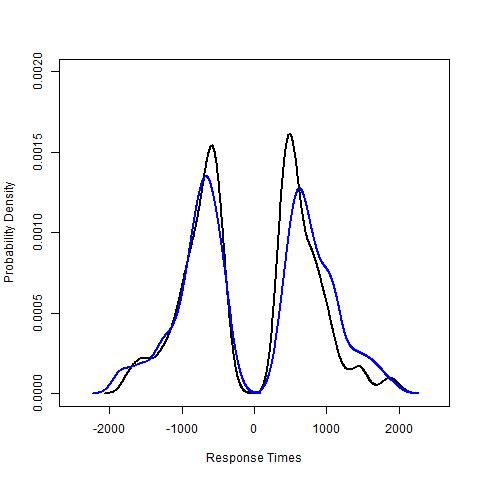
\includegraphics[width=0.9\textwidth]{Cond_distr_RRdata}
\caption{Estimated correct and error probability densities of response times. Positive response times correspond to correct choices and negative response times to incorrect choices. Black line is subject ``nh'' and blue line is subject ``jf''. }
\label{fig:conddist}
\end{figure}
%

Another central feature of behavioral data is asymmetry between correct and error responses. It may be seen in Figure \ref{fig:conddist}, especially with error means being slower than correct means, which is typical for difficult stimulus conditions \citep{Swe1972}. However, a more complete understanding of relation between correct and error response times arises from examining performance across several difficulty and instruction combinations. One effective graphical summary that can reveal relations between correct and error response times is called a latency-probability graph (LPG). LPG is a function that maps proportions of correct or error responses into mean response times, thus tracking stimulus difficulty conditions \citep{RatRou1998}.

Figure \ref{fig:lpg} shows a plot of a LPG for one subject presented with stimuli of different brightness, either under speed or accuracy instructions. When accuracy was emphasized, the subject showed faster errors for easy stimuli (really bright or dark) and slow errors for difficult stimuli relative to correct responses. When instructions shift to ``speed'' the asymmetry is strongly reduced or vanishes \cite{Vic1979}.  

Another pattern that is ubiquitous in behavioral data is the speed-accuracy trade off obtained by manipulating instructions \citep{Vic1979, Luc1986, Hei2014}. Instructing a subject to emphasize accuracy instead of speed results in shifting and rescaling both correct and error densities towards slower response times. The effect is obvious in Figure \ref{fig:lpg} with the LPG shifting upwards and to the right when instructions are changed from ``accuracy'' to ``speed''. 

In contrast to the speed-accuracy trade-off under instructions, concentrating on either the speed or accuracy condition, the relation between response times and accuracy is different. Figure \ref{fig:lpg} shows that the higher accuracy the faster the subject responds. Intuitively, when stimulus gets easier the subject is more accurate and is faster.

\begin{figure}
\centering
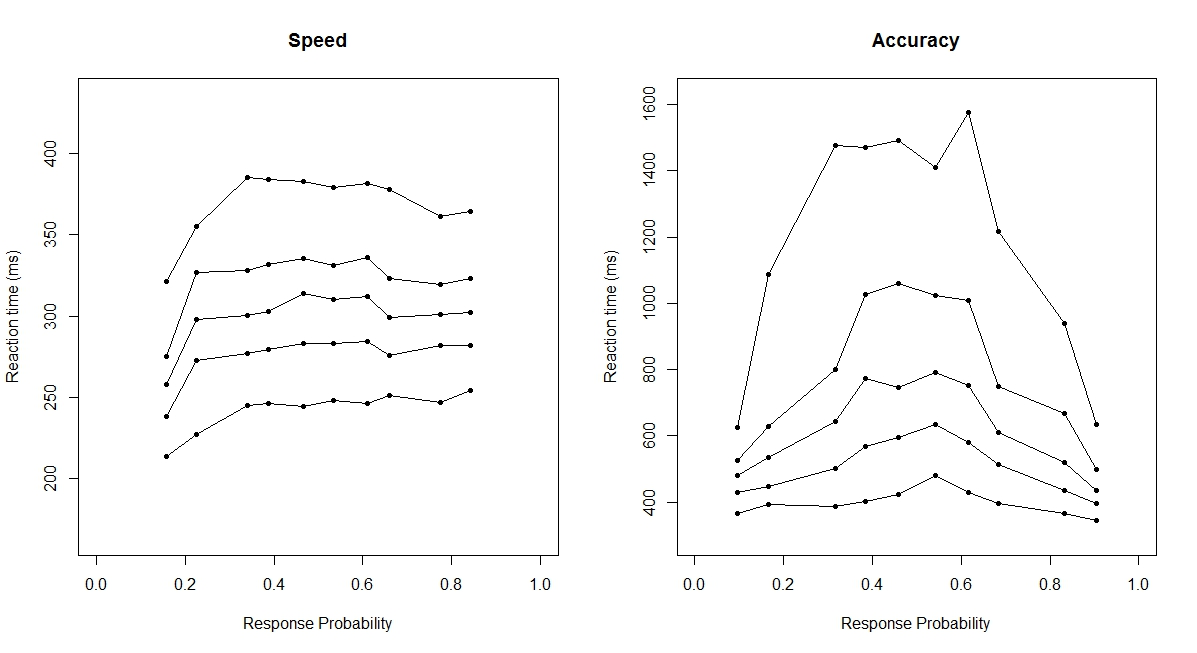
\includegraphics[width=0.9\textwidth]{QP_RRdata}
\caption{Latency-probability plot. Below 0.5 are error rates and above 0.5 are correct rates. Points represent a summary of performance with lines drawn to capture a trend. The lower line is due to speed emphasis and the upper line is due to accuracy emphasis.}
\label{fig:lpg}
\end{figure}
%

The last two aspects of the benchmark data are shown in Figure \ref{fig:autoacf}. The plot is based on response times collected in two consequtive blocks under speed instruction. Similar data features appear in other blocks. The first feature is presence of extreme response times. For example, the Trial Series subplot shows that response nine took 538 ms, and response 21 lasted 196 ms. Relative to the rest of the responses, these have extreme duration. Presence of extreme observations may indicate genuine response times from tails of the distribution carrying information about processing of interest, but it is not completely clear \citep{CraPer2010}.

The second feature is portrayed in the Auto-correlation subplot of Figure \ref{fig:autoacf}. The dotted blue line represents a critical value for an alpha-level of 0.05 hypothesis test of zero auto-correlation. Data from the selected block is consistent with auto-correlation between response times stretching 6 trials. 

%
\begin{figure}
\centering
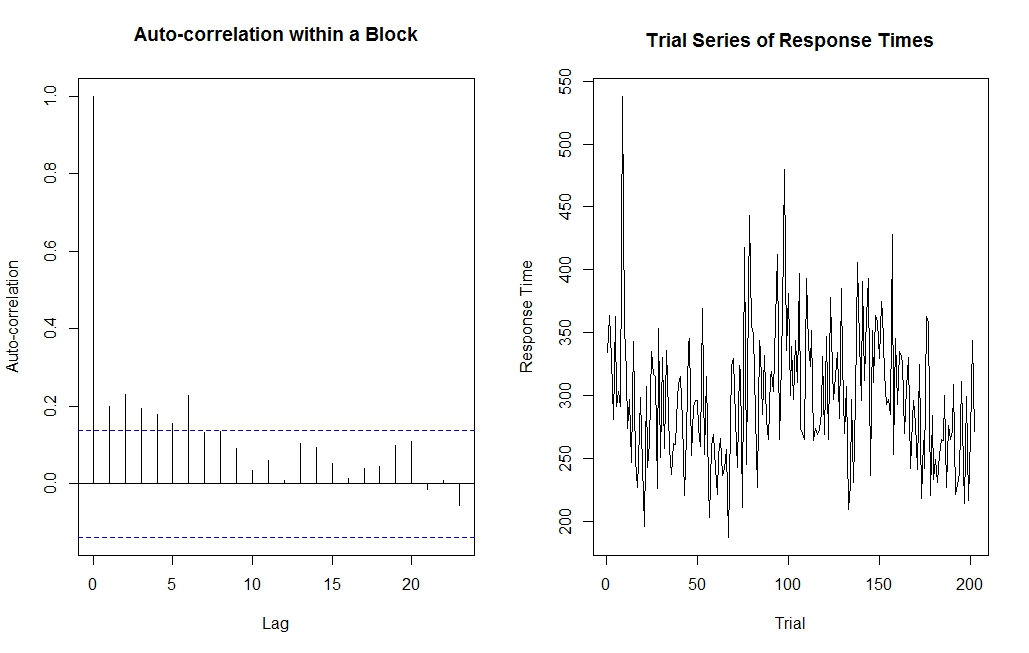
\includegraphics[width=0.9\textwidth]{Auto_Acf_RRdata}
\caption{Auto-correlation function and trial series of response times. Values above the dotted line represent significant auto-correlation.}
\label{fig:autoacf}
\end{figure}
%

The complete pattern of data features including speed-accuracy tradeoff, amount of variation in response times, skew of the conditional densities, relation between correct and error response times, relation between response time and accuracy, extreme response times and auto-correlation in response times provides strong constraints for developing and testing models of decisions. In the next section, I will discuss a promiment theoretical framework for understanding simple choice behavior and how it gets implemented in testable models.


%%%%%%%%%%%%%%%%%%%%%%%%%%%%%%%%%%%%%%%%%%%%%%%%%%%%%%
\section{Theoretical Data Models}
%%%%%%%%%%%%%%%%%%%%%%%%%%%%%%%%%%%%%%%%%%%%%%%%%%%%%%

A common approach to conceptualizing cognitive processing underlying two-choice
tasks is to decompose them into processes of encoding of stimulus features, response selection based on a relevant stimulus feature and motor execution. A cognitive process model for these tasks should make sufficient assumptions about these processes to predict patterns in performance
data. A delicate balance has to be struck between what processing details to include
and what details to exclude from models because it will determine their generalizability across two-choice tasks. For instance, including details about how lexical information is accessed in
memory to direct response selection will make a model inapplicable to
brightness discrimination. The dominant approach to this balancing problem
is sequential sampling framework.
    
A fundamental theoretical assumption of the sequential sampling framework
is that the same general decision process operates across all two-choice
tasks. Then, a generalizable model should provide a detailed account of the
decision process while making simplifying assumptions about the stimulus encoding
and motor processing, like assuming a constant non-decision time. Over the last $\sim50$ years, many models of this type
have been developed \citep{Sto1960,Rat1978,Vic1979,RatTue2002,Smi1995,UshMcc2001,BroHea2008}. Some of the most successful ones
can explain many patterns in the response time and response data,
under a variety of experimental conditions and tasks
\citep{RatSmi2004,Wag2009}.
    
The underlying principle of sequential sampling models is that when an
observer is tasked with selecting a correct response in limited time
from a noisy stimulus, he or she accumulates samples of 
information from the relevant stimulus attribute representation until one of two
decision thresholds is reached
\citep{Vic1979,TowAsh1983,Luc1986,BogBro2006}. The structure of thresholded accumulation enables to unite concepts of decision bias, caution and information quality under a single mechanism. Differential levels of initial information produce bias, thresholds control caution and rate of information uptake reflects information quality. Combination of these variables in thresholded accumulation also naturally predict decisions and times. The time taken to reach a threshold and the crossed threshold map onto decision time and decision. The sequential sampling principle is powerful, but to connect it to behavioral data we need a model. 
    
Given the sequential sampling principle, any concrete model of simple decisions makes detailed assumptions about the nature of sampled
information, temporal structure of sampling, stopping rule and sources of
randomness \citep{Vic1979,RatSmi2004,BogBro2006,TeoUsh2013}. For example, sampled information can consist of discrete or
continuous packets. The size of packets may be fixed or variable. The
accumulation of information packets may happen at fixed or variable
discrete time points, or continuously. The stopping rule may be absolute,
in which case accumulation stops when evidence in favor of one of the
choices reaches a threshold, regardless of the amount of evidence favoring
the alternative. In contrast, a relative rule requires that evidence
favoring one of the choices has to exceed the other by some amount. Finally, models vary in whether starting points, rate of information uptake or thresholds vary across trials. Combinations of
modeling assumptions generate the range of possible sequential sampling
models.
    
Examples of sequential sampling models include a random walk model that
stops accumulation of discrete packets of information over
discrete time steps according to a relative rule \citep{Lam1968}, a Poisson
counter model that describes accumulation of discrete, fixed information
packets arriving at random time points until evidence for either of the choices reaches a threshold
\citep{TowAsh1983}, and a Wiener diffusion model that describes accumulation
of continuous packets in continuous time until a relative threshold is hit
\citep{Rat1978}. 

In addition to assumptions about the accumulation process, models also add assumptions about variability in their parameters across trials. For example, an early random walk model assumed variability in starting points \citep{Lam1968}, a version of a Poisson counter model reported in \citet{RatSmi2004} added variability in the rate of information uptake and thresholds, and a popular version of a Wiener diffusion  model incorporates variability in starting points, rate of information uptake and non-decision time.

The sequential sampling framework has been fruitful in providing models that could be used to investigate correlations between parameters. The assumptions of a particular model lead to a precise prediction of how response times and responses jointly vary \citep{RatSmi2004}. The joint density can be used as a theoretically motivated data model in statistical analysis of behavioral data. In the next section, I will characterize Bayesian statistical framework that allows a principled and intuitive way for extracting information about the supposed latent decision process from behavioral data.

%%%%%%%%%%%%%%%%%%%%%%%%%%%%%%%%%%%%%%%%%%%%%%%%%%%%%%%%
\section{Bayesian Statistical Framework}
%%%%%%%%%%%%%%%%%%%%%%%%%%%%%%%%%%%%%%%%%%%%%%%%%%%%%%%%

Once we form a model of behavioral data, how should we use the data? In the following subsections, I will present a Bayesian hierarchical framework and a fitting method based on Markov chains that can provide a formal approach to examining generalized models of simple choice behavior \citep{Ber1997,CasBer2002,GelCar2013}. In the Bayesian framework a model of data is combined with a model of unknown parameters to provide a combined description of uncertainty. While theoretically everything tends to work out beatifully, in practice Bayesian models with complex data distributions are usually analytically intractable and require an iterative algorithm, often called a sampler, to learn about parameters and the model(s) from data. 

Recent developments in computing power and software made the Bayesian approach ripe for
scientific use \citep{Kru2010}, and it is becoming popular in psychology, too
\citep{EdwLin1963,MyuPit1997,PerVan2002,RouLu2005,RouLu22005,MyuKar2008,CraPer2010,VanTue2011,LeeWag2014}. The
reasons for its appeal include quantifying of uncertainty with
probability, making statistical inferences as probability statements and ability to fit realistic models. On these grounds, I will adopt Bayesian approach to a data analysis study specified below, but before that I will present the fundamental ideas of hierarchical modeling and Markov Chain Monte Carlo.

%%%%%%%%%%%%%%%%%%%%%%%%%%%%%%%%%%%%%%%%%%%%%%%%%%%%%%%
\subsection{Bayesian Hierarchical Models}		
%%%%%%%%%%%%%%%%%%%%%%%%%%%%%%%%%%%%%%%%%%%%%%%%%%%%%%%

In the Bayesian framework model parameters are treated as random variables
along with data. The full probability model, also called the Bayesian
model, is at the center of analysis because all inference problems can be defined in terms of it
\citep{GelCar2013}. A Bayesian model requires specifying
the probability densities of both data and
parameters. The probability densities are assumed to be conditionally dependent in a way that the full joint density can
be factored into a probability density of data given parameters,
called a sampling density, and the probability density of parameters,
called a prior density. Given a data vector $\boldsymbol{x} \in \mathbb{R}^p$ and
its parameter vector $\boldsymbol{\theta} \in \Theta \subseteq
\mathbb{R}^m$, a Bayesian model is written as
%
\begin{equation}
\label{eqn:bayesmodel}
f(\boldsymbol{x}, \boldsymbol{\theta}) =
      f(\boldsymbol{x} \mid \boldsymbol{\theta})\pi(\boldsymbol{\theta}) 
\end{equation} 
%
where $f(\boldsymbol{x} \mid \boldsymbol{\theta})$ is a sampling density and $\pi(\boldsymbol{\theta})$ is a prior density for
$\boldsymbol{\theta}$. The ability to factor a joint density of
$\boldsymbol{x}$ and $\boldsymbol{\theta}$ into a sampling and a prior density is
useful for constructing new Bayesian models because it allows breaking
the problem into manageable pieces, often consisting of common
univariate distributions \citep{JohKot1994,JohKot1995}.

Statistical inference proceeds by conditioning unknown quantities of interest on the observed data $\boldsymbol{x}$. For example, estimation of parameters $\boldsymbol{\theta}$ amounts to calculating a posterior density $\pi(\boldsymbol{\theta} \mid \boldsymbol{x})$, which contains all the information about the parameters, using the Bayes' theorem
% 
\begin{equation} 
\label{eqn:posterior}
\pi(\boldsymbol{\theta} \mid \boldsymbol{x}) = 
   \frac{f(\boldsymbol{x} \mid \boldsymbol{\theta}) \pi(\boldsymbol{\theta})} 
        {\idotsint\limits_\Theta f(\boldsymbol{x} \mid \boldsymbol{\theta})
         \pi(\boldsymbol{\theta})d\boldsymbol{\theta}}
\end{equation} 
% 
\citep{Ber1997,CasBer2002,Ber2011,GelCar2013}. We can then extract more specific probability statements about $\boldsymbol{\theta}$ from the posterior density such as $P(\boldsymbol{\theta} \in A \mid \boldsymbol{x})$, where $A \subseteq \Theta$. 

The expression in Equation \ref{eqn:bayesmodel} suggests a situation where a set of observations all come from the same source and can be used to infer something about common parameters. However, the structure of behavioral data is rather different. A typical experiment generates
multiple observations for each of several participants engaged in the
same task \citep{RatMck2008,Wag2009}. When specifying a statistical
model, the experimenter must choose whether to treat individual observations as coming from different distributions, ``no pooling'' model, or the same distribution, ``complete pooling'' model \citep{RouLu2005,RouLu22005,RouMor2014}. 

Not pooling the data presupposes no relation between the individuals while completely
pooling data ignores individual differences. However, for human
behavioral data, it is more accurate to assume a middle ground. Real
data varies among participants, but due to similarity in cognitive
abilities and experimental treatment, participants share regularities. A hierarchical statistical model acknowledges this mixed
structure by assuming that individual parameters are a random sample
from a population with data nested within each individual, and thus introduces
``semi-pooling'' of information by fitting all the data simultaneously \citep{GelCar2013}. Hence, I propose treating  sequential sampling models under consideration in a hierarchical fashion \citep{Ber1997,GelCar2013,RouLu2005,CraPer2010}. 

There is no rigorous definition of a hierarchical model, but it is often considered that a model with at least two levels of parameters qualifies as hierarchial. In the simplest case, the parameter space can be factored
into first-level parameters representing individuals and
second-level parameters representing a population from which
individuals' parameters are sampled.  With data $\boldsymbol{x} \in \mathbb{R}^p$
conditionally dependent on the first-level parameters $\boldsymbol{\theta} \in \Theta
\subseteq \mathbb{R}^m$, and first-level parameters conditionally dependent on
second-level parameters $\boldsymbol{\psi} \in \Psi \subseteq \mathbb{R}^n$, a two-level
hierarchical model can be stated as
%
\begin{equation}
f(\boldsymbol{x}, \boldsymbol{\theta}, \boldsymbol{\psi}) =
f(\boldsymbol{x} \mid \boldsymbol{\theta})
f(\boldsymbol{\theta} \mid \boldsymbol{\psi})
f(\boldsymbol{\psi}).
\end{equation}
%
In words, a joint density over data and all parameters can be factored into a sampling density $f(\boldsymbol{x} \mid
\boldsymbol{\theta})$, a first-level prior density of parameters $\pi(\boldsymbol{\theta} \mid
\boldsymbol{\psi})$ and a second-level prior density of parameters $f(\boldsymbol{\psi})$. In the context of sequential sampling models, a density over a collection of responses and response times is a sampling density, a density over individual's correlation parameter between bias and non-decision time, say, is the first-level prior and a density over the correlation parameter is the second-level prior. Combining all the data together hierarchically and then conditioning on all of it will lead to improved estimation of important cognitively interpretable parameters of each individual because data is shared across individuals, which is sometimes called a shrinkage effect \citep{GelCar2013}.

While hierarchical Bayesian models have many advantages, one typical simplifying assumption taken when using hierarchical models, which I will adopt, is exchangeability of observations. A sequence of random variables $\{x_1, x_2, ..., x_n\}$ is exchangeable when 
\begin{equation}
f(x_1, x_2, ..., x_n) = f(x_{z(1)}, x_{z(2)}, ..., x_{z(n)}),
\end{equation}
for all permutations z over $\{1, 2, ...,n\}$ \citep{GelCar2013}. In other words, order indeces of random variables carry no information about them. The consequence of exchangibility is that conditional on first level parameters $\boldsymbol{\theta}$, observations are independent and a prior for $\boldsymbol{\theta}$ exists, formally justifying Bayesian analysis. Exchangeability is a simplifying assumption because actual response times have autocorrelation structure that is altered by permutations, as can be seen in Figure \ref{fig:autoacf}. However, numerous successful fits of sequential sampling models suggest that exchangeability is a reasonable simplification \citep{UshMcc2001,RatSmi2004,RatMck2008}.

To conclude, the joint density over observations and all parameters is the starting point of Bayesian analysis. I will use a hierarchical modeling approach to capture the patterns of similarities and differences between humans performing simple decision tasks, while simplifying the models with assumption of exchangeability. However, the models I will define are still too complex for analytical treatment, which brings us to the topic of how complicating the situation with Markov chains actually enables practical application of Bayesian inference.


%%%%%%%%%%%%%%%%%%%%%%%%%%%%%%%%%%%%%%%%%%%%%%%%%%%%%%%
\subsection{MCMC Background}
%%%%%%%%%%%%%%%%%%%%%%%%%%%%%%%%%%%%%%%%%%%%%%%%%%%%%%%

After a Bayesian model has been specified, inference about
parameters, out-of-sample observations or the model can proceed by applying the calculus of
probabilities to obtain corresponding conditional densities. With continuous parameters, which is the typical case, calculating conditional densities requires integration, which for complex models is intractable. Application of Bayes' theorem to obtain a posterior density over unknown quantities is
complicated by the integral in the denominator of
Equation \ref{eqn:posterior}. In particular, the inability to integrate over parameters relative to appropriate parameter density plagues the best sequential sampling models, so the
posterior density cannot be calculated exactly \citep{RouLu2005,VanTue2011}. 

Due to high-dimensionality of Bayesian models, numerical integration techniques fall apart leaving Monte Carlo methods as the only viable option. Monte Carlo methods rely on simulating pseudo-random draws from a distribution of interest to solve inference problems. For data models with known mathematical form, approximate inferences can be obtained through a 
special class of Monte Carlo algorithms, sometimes called samplers, that use Markov chains (MCMC) to sample from posterior densities
\citep{RobCas2004,GamLop2006,GivHoe2012,GelCar2013}. Given a posterior sample, accurate conclusions can be drawn, even for complicated models
\citep{PerVan2002,CraPer2010,VanTue2011}. In the rest of the section, I will present a few definitions from Markov chain theory as background for a general class of MCMC algorithms built on that theory.

MCMC employs discrete-time, continuous state space Markov chain to sample from arbitrary distributions
for which a probability density can be specified \citep{KarTay1975,KarTay1981,Ros2014}. Let $\boldsymbol{X} = \{\boldsymbol{x}_n: n \geq 0\}$ be a p-dimensional, discrete-time stochastic process with state space $\mathcal{S} \subseteq \mathbb{R}^p$. A first-order Markov chain is a stochastic process with a conditional distribution satisfying
\begin{equation}
f(\boldsymbol{x}_n \mid \boldsymbol{x}_{n-1}, \boldsymbol{x}_{n-2}, \ldots, \boldsymbol{x}_0) = f(\boldsymbol{x}_n \mid \boldsymbol{x}_{n-1}),
\end{equation}
for any $n \geq 1$.
In words, the distribution of a current state depends only on the previous state, giving Markov chains a memoryless property. 

A Markov chain $\boldsymbol{X}$ can be thought of as a model of stochastic dynamics of a multi-dimensional system over discrete time. Description of dynamics requires an initial position in the state space and a transition rule that guides the system from state to state. Given that $\mathcal{S}$ is continuous and $\boldsymbol{X}$ is stochastic, description of the process requires a marginal density of $\boldsymbol{x}_0$, called an initial density, and a conditional density of $\boldsymbol{x}_n$ given $\boldsymbol{x}_{n-1}$, called a transition density. Once densities descibing dynamics are defined, evolution of the process can be analyzed analytically or through simulation.

It can be shown that some Markov chains, if given enough time, will go from an arbitrary initial density to an equilibrium density. Equilibrium behavior is a property of a transition density. For a transition density $f(\boldsymbol{x}_n \mid \boldsymbol{x}_{n-1})$ and $A \subseteq S$, a transition kernel is defined as
\begin{equation}
P\{\boldsymbol{x}_n \in A \mid \boldsymbol{x}_{n-1}\} = \int_A f(\boldsymbol{x}_n \mid \boldsymbol{x}_{n-1})d\boldsymbol{x}_n.
\end{equation}
Starting from any point $\boldsymbol{x}_0 \in S$, a Markov chain has an equilibrium density if an nth-step transition kernel converges satisfies
\begin{equation}
\lim_{n \to \infty}P(\boldsymbol{x}_n \in A \mid \boldsymbol{x}_{0}) = \pi(A),
\end{equation}
where $\pi(\cdot)$ is called an equilibrium density function. 

Once a chain attains equilibrium behavior, whatever the initial position is and no matter how many transitions occur after, the chain remains in equilibrium. The sequence of states $\boldsymbol{x}_n, \boldsymbol{x}_{n+1}, \ldots$ will be identically distributed according to the equilibrium density function. The equilibrium behavior provides a natural point of contact with the problem of Bayesian inference for complex models. If the equilibrium density is equivalent to the posterior density, then a sample of states of a Markov chain in equilibrium is a sample from the posterior. 

It follows then that Bayesian analysis can proceed if a Markov chain can be simulated for which there exists a unique equilibrium density equivalent to the posterior density that can be reached from an arbitrary starting point. The limit-based definition of the equilibrium density implies that it is not guaranteed to exist nor to be unique. Four conditions need to be satisfied to obtain the desired subclass of Markov chains. 

First, a Markov chain has to be homogeneous. Homogeneity is  defined by a time-invariant transition density, such that
\begin{equation}
f(\boldsymbol{x}_n \mid \boldsymbol{x}_{n-1}) = f(\boldsymbol{x}_1 \mid \boldsymbol{x}_0),
\end{equation}
for any $n \geq 1$. A homogeneous chain has fixed dynamics across time, but marginal densities $f(\boldsymbol{x}_n)$ are not guaranteed to be equal across time nor is there a guarantee that marginal densities converge to an equilibrium density. Homogeneity is a flexibixibility condition allowing different initial densities and setting up a possibility of convergence to an equilibrium density. 

Homogeneous Markov chains have to constrained further to ensure convergence to a unique equilibrium density. The second requirement is that a Markov chain is $\phi$-irreducible.  Let the time of first re-visit to $A$ from $\boldsymbol{x_0}$ be a random variable $t_A = \inf_{n \geq 1} \{\boldsymbol{x}_n \in A\}$, where set $A \in S$ and starting point $\boldsymbol{x}_0 \in A$. A Markov chain is $\phi$-irreducible if there exists a marginal density $f(\cdot)$, such that for all $\boldsymbol{x}_0 \in A$ and all $A \in S$, 
\begin{equation}
P\{t_A < \infty \mid \boldsymbol{x}_0\} > 0. 
\end{equation}
$\phi$-irreducibility ensures that no matter where the chain starts it is possible to return there in finite amount of time. In other words, there are no regions where a chain gets stuck, which would create a possibility for multiple equilibrium densities.

In addition to moving around the state space without getting stuck in some region, a chain should also have no cyclical behavior. The third required property of chains with unique equilibrium density is aperiodicity. An aperiodic Markov chain can move from any $A \subseteq S$ back to $A$ in one transition, that is for $n \geq 1$ and $\boldsymbol{x}_{n-1} \in A$
\begin{equation}
P\{\boldsymbol{x}_n \in A \mid \boldsymbol{x}_{n-1}\} > 0. 
\end{equation}
As a result, an aperiodic chain can explore the same region without leaving it. 

The first three properties ensure that a Markov chain converges to a unique equilibrium density from most initial positions. To ensure that a process converges from all initial positions, it must be Harris recurrent. For $A \subseteq S$ with $\pi(A) > 0$ and all $\boldsymbol{x} \in A$, a $\phi$-irreducible Markov process with an equilibrium density $\pi(\cdot)$ is Harris recurrent if 
\begin{equation}
P\{t_A < \infty \mid \boldsymbol{x}_0\} = 1.
\end{equation}
Harris recurrence guarantees that all realized chains come back to the region where they start in finite amount of time.

Recall that we started with a problem of statistical inference with complex Bayesian models that can be solved with Monte Carlo methods. Conditions of homogeneity, $\phi$-irreducibility, aperiodicity and Harris-recurrence are sufficient to guarantee that a proposed MCMC algorithm can solve intractable integrals in Bayesian inference. The next issue we consider is how to find such algorithms.

%%%%%%%%%%%%%%%%%%%%%%%%%%%%%%%%%%%%%%%%%%%%%%%%%%%%%
\subsection{Metropolis-Hastings Algorithm}
%%%%%%%%%%%%%%%%%%%%%%%%%%%%%%%%%%%%%%%%%%%%%%%%%%%%%

The Markov chain theory on its own provides only conditions that a valid algorithm should satisfy, but gives no clues of a working algorithm. As opposed to analysis in probability theory where having a transition density and figuring out its equilibrium density is the problem, in Bayesian analysis the equilibrium density is known and a transition density needs to be figured out. A very general way for constructing transition densities is a class of algorithms called Metropolis-Hastings \citep{RobCas2004,GivHoe2012,GelCar2013}. The algorithm provides a way to define a transition density satisfying the four properties required for a Markov chain to converge to a known equilibrium density from an appropriate initial density. 

In the situation where MCMC methods apply, we are in possession of a target density, $\pi(\cdot)$. We need a transition density, $p(\boldsymbol{y} \mid \boldsymbol{x})$ (or the associated transition kernel), whose equilibrium density is $\pi(\cdot)$. A sufficient condition for $p(\boldsymbol{y} \mid \boldsymbol{x})$ to be a proper transition density is called detailed balance (also called time reversibility), 
\begin{equation}
\pi(\boldsymbol{x})p(\boldsymbol{y} \mid \boldsymbol{x}) = \pi(\boldsymbol{y})p(\boldsymbol{x} \mid \boldsymbol{y}).
\end{equation}
Detailed balance says that starting at $\boldsymbol{x}$ and moving to $\boldsymbol{y}$ happens as often as starting at $\boldsymbol{y}$ and moving to $\boldsymbol{x}$. In addition, if the transition density $p(\boldsymbol{y} \mid \boldsymbol{x})$ has support equal to $\pi(\cdot)$ or contained in it, then it will satisfy properties of homogeneity, $\phi$-irreversibility, aperiodicty and Harris recurrence, ensuring convergence from any starting point in the state space to a unique equilibrium density. 

Naive or ad-hoc methods for constructing a transition density are likely not to satisfy detailed balance, except for maybe special cases, but their failure is instructive. When a method fails to satisfy detailed balance it implies that, for some combinations of $\boldsymbol{x}$ and $\boldsymbol{y}$, $\pi(\boldsymbol{x})p(\boldsymbol{y} \mid \boldsymbol{x}) > \pi(\boldsymbol{y})p(\boldsymbol{x} \mid \boldsymbol{y})$ or the reverse. Loosely, the chain moves too frequently from $\boldsymbol{x}$ to $\boldsymbol{y}$ and rarely from $\boldsymbol{y}$ to $\boldsymbol{x}$. The Metropolis-Hastings algorithm is a general approach to MCMC algorithms that provides a way to correct the imbalance by introducing a possibility that a transition may be rejected.

Suppose the chain at time $n - 1$ is in state $\boldsymbol{x}_{n-1} = \boldsymbol{x}$. For a move to take place, a Metropolis-Hastings algorithm requires a proposal density $q(\boldsymbol{y} \mid \boldsymbol{x})$ from which a candidate value can be drawn. A candidate value is then accepted with probability $\alpha(\boldsymbol{y}, \boldsymbol{x})$, called acceptance probability. The transition density in a situation when the chain moves ($\boldsymbol{x}_n = \boldsymbol{y}$) is
\begin{equation}
q(\boldsymbol{y} \mid \boldsymbol{x})\alpha(\boldsymbol{y}, \boldsymbol{x}).
\end{equation}
In a situation where the chain does not move ($\boldsymbol{x}_n = \boldsymbol{x_{n-1}})$, there is a probability mass at $\boldsymbol{x}$,
\begin{equation}
r(\boldsymbol{x}) = 1 - \int_S q(\boldsymbol{y} \mid \boldsymbol{x})\alpha(\boldsymbol{y}, \boldsymbol{x})d\boldsymbol{y},
\end{equation}
with integral accounting for all possible moves. 
Combining the two pieces, for $d\boldsymbol{y} \subseteq S$ and $\boldsymbol{x} \in S$, the transition kernel of Metropolis-Hastings chain is
\begin{equation}
P\{\boldsymbol{x}_n \in d\boldsymbol{y} \mid \boldsymbol{x}_{n-1}\} = q(\boldsymbol{y} \mid \boldsymbol{x})\alpha(\boldsymbol{y}, \boldsymbol{x})d\boldsymbol{y} + r(\boldsymbol{x})\delta_{\boldsymbol{x}}(dy),
\end{equation}
where $q(\boldsymbol{y} \mid \boldsymbol{x}) = 0$ when $\boldsymbol{y} = \boldsymbol{x}$, and Dirac's $\delta_{\boldsymbol{x}}(d\boldsymbol{y}) = 1$ when $\boldsymbol{x} = \boldsymbol{y}$ and 0 otherwise. 

The final part of the algorithm is the definition of acceptance probability. From considering the two kinds of inequalities that violate the detailed balance condition, acceptance probability for moving from $\boldsymbol{x}$ to proposed $\boldsymbol{y}$ is derived to be
%
\[
\alpha(\boldsymbol{y}, \boldsymbol{x}) =
\begin{dcases}
\min\left(\frac{\pi(\boldsymbol{x})q(\boldsymbol{y} \mid \boldsymbol{x})}{\pi(\boldsymbol{y})q(\boldsymbol{x} \mid \boldsymbol{y})},1\right) & : \pi(\boldsymbol{y})q(\boldsymbol{x} \mid \boldsymbol{y}) > 0 \\
1 & : \pi(\boldsymbol{y})q(\boldsymbol{x} \mid \boldsymbol{y}) = 0
\end{dcases}
\]
%
The form of $\alpha(\boldsymbol{y}, \boldsymbol{x})$ implies that the target density needs to be known only upto a normalizing constant because it cancels out in the fraction. The cancelation of normalizing constants is directly relevant for Bayesian inference because these constants are the intractable integrals. The form also implies that the algorithm always moves to places of higher probability density, but moves to places of lower probability with some probability. Algorithm \ref{fig:mh} shows Metropolis-Hastings pseudocode for sampling N draws from a target density $\pi(\cdot)$.

\begin{algorithm}
\centering
\begin{algorithmic}
\State Initialize at $\boldsymbol{x}_0 \ni 						   \pi(\boldsymbol{x}_0) > 0$
\For {$j = 1, 2, \ldots, N$} 
  \State Sample $\boldsymbol{y} \sim q(\boldsymbol{y} \mid 			 \boldsymbol{x}_{j-1})$
  \State Sample $u \sim \mathcal{U}(0, 1)$
  \If {$\alpha(\boldsymbol{y}, \boldsymbol{x}_{j-1}) \geq u$}
    \State Set $\boldsymbol{x}_j = \boldsymbol{y}$
  \Else 
    \State Set $\boldsymbol{x}_j = \boldsymbol{x}_{j-1}$
  \EndIf
\EndFor
\end{algorithmic}
\caption{\label{fig:mh} Metropolis-Hastings Pseudocode}
\end{algorithm}

%%%%%%%%%%%%%%%%%%%%%%%%%%%%%%%%%%%%%%%%%%%%%%%%%%%%%%%%%%%%%%%
\chapter{Questions to be Answered}
%%%%%%%%%%%%%%%%%%%%%%%%%%%%%%%%%%%%%%%%%%%%%%%%%%%%%%%%%%%%%%%

In the first chapter I raised some questions about dependent adjustment in parameters of cognitive processes underlying simple choice behavior. I presented some behavioral and modeling evidence for it, and reviewed a theoretical and statistical framework within which answers to these questions may be sought.  In this chapter, I will elaborate on questions to be addressed by this thesis. There are three overaching questions that I propose to pursue: How to incorporate trial-to-trial dependencies between parameters into models of cognitive processes underlying behavior on two-choice tasks? How do predictions of cognitive models change under assumption of dependence relative to independence of parameters? What information about dependencies between parameters, given some sequential sampling model of the decision process, does the benchmark dataset have?

%%%%%%%%%%%%%%%%%%%%%%%%%%%%%%%%%%%%%%%%%%%%%%%%%%%%%%%%%%%%%%%%%
\section{Modeling Parameter Dependencies}
%%%%%%%%%%%%%%%%%%%%%%%%%%%%%%%%%%%%%%%%%%%%%%%%%%%%%%%%%%%%%%%%%

One of the main questions underlying this thesis is how to formally describe coordination of cognitive processes across trials. However, before stating the question in an answerable form, lets consider the bigger picture. Recall that behavioral and modeling data suggest that across trials parameters that capture underlying processes show both auto-correlation and cross-correlation. As a final target of research we may consider finding a system of equations that can describe such dynamics in a way that reflects a mechanistic theory. Suppose we are dealing with a sequential sampling model of binary choice that has some initial evidence $\xi$, rate of evidence accumulation $\delta$, threshold separation $\alpha$ and non-decision time $\tau$. On each trial a participant generates a response time $t^{rt}$ and a response r. Then, change in the task-specific processing from trial $n$ to $n+1$ may be captured by the following dynamic system:
%
\begin{eqnarray}
\alpha(n+1) = f_{\alpha}(\alpha(n), t^{rt}(n), r(n),\theta_{\alpha}), \nonumber \\
\xi(n+1) = f_{\xi}(\xi(n), t^{rt}(n), r(n),\theta_{\xi}), \nonumber \\
\delta(n+1) = f_{\delta}(\delta(n), t^{rt}(n), r(n),\theta_{\delta}), \text{and} \nonumber \\
\tau(n+1) = f_{\tau}(\tau(n), t^{rt}(n), r(n),\theta_{\tau}).
\end{eqnarray}
%
The dependence of parameters at trial $n + 1$ on themselves at trial $n$ and other stable processes captured by $\theta_i$ can explain first-order auto-correlation, and dependence on previous choice and its speed can explain cross-correlations. 

There have been some quantitative proposals that capture auto-correlation of some parameters across trials, which is a special case of the above system \citep{Lam1968,Vic1979,Luc1986,ChoNys2002,BroMar2008,GaoWon2009,GolWon2012}. The thrust of this work relies on the rich pattern of sequential effects that provide suggestive constraints on dynamic rules for various parameters. For example,\citet{GolWon2012} examined post-error slowing and suggested a dynamic rule for threshold separation that leads to increases after error and decreases after correct responses. Another suggestive sequential effect is speed up of correct responses on the second repeating stimulus with short response-to-stimulus interval, which \citet{GaoWon2009} described with a bias in the starting evidence towards the correct boundary. 

However, when it comes to cross-correlations of parameters, the behavioral data is less clear and I found no explicit modeling studies of cross-correlations. Based on these suppositions, I propose to study cross-correlations among parameters from a descriptive rather than a mechanistic perspective. Instead of specifying dynamic rules for all or some of the parameters to impose dependencies, I can replace assumptions of independent variation of the standard models with dependent variation. Dependent variation can be specified as a multivariate distribution that provides means and scales as the standard models, but also adds correlations between parameters. The magnitude and direction of correlations between different pairs of parameters could then suggest a target for a comprehensive mechanistic theory expressed in a system of dynamic equations.
    
By formalizing parameter relations in a statistical manner, the first question can now be formulated more concretely: what multivariate density should model joint variation among parameters across trials? Couple of key properties of standard sequential sampling models provide important constraints on the search space. One feature of all standard models is that parameters fall on different scales. Rates of evidence uptake take values from $\mathbb{R}$, evidence thresholds are positive and initial evidence may fall between 0 and evidence threshold \citep{RatSmi2004}. In addition, probability density functions that we assign to each parameter may all be different to reflect different kind of marginal variation \citep{Rat2013,JonDzh2014}. 

The combination of scales and marginal densities restrictions may be hard to satisfy with common multivariate densities. There is a stock of multivariate densities that could be used to model dependence in certain situations, including the normal, t, gamma, and F \citep{KotBal2004}. However, they are too restricted in their properties to be used for generalizing sequential sampling models. For example, in each of the commonly used densities the support of each dimension is the same and so are the marginal densities. A n-dimensional multivariate normal has support over $\mathbb{R}^n$ and each marginal is a normal density with some mean and variance. These considerations suggest that we need a method for defining new multivariate densities that fit the above restrictions and express alternative correlation structure.

%%%%%%%%%%%%%%%%%%%%%%%%%%%%%%%%%%%%%%%%%%%%%%%%%%%%%%%%%%%%%%%%
\section{Predictions of Dependent Parameters}
%%%%%%%%%%%%%%%%%%%%%%%%%%%%%%%%%%%%%%%%%%%%%%%%%%%%%%%%%%%%%%%%

Assuming we have specified a joint distribution of parameters, we can now ask what are the consequences of dependent parameters. Predictions made by models is a natural way of understanding what model assumptions imply. Comparison of a model with dependent parameters to a model with independent parameters can reveal how different trade-off patterns between parameters shape the decision process and provide insight into which data patterns indicate dependent parameters. The result of this should be a better understanding of how a decision process with parameters changing across trials in a coordinated manner differs from the usually assumed process with independent parameters.

Sequential sampling models of a simple decision process provide two avenues for understanding implications of correlated parameters. On the one hand, since sequential sampling models are dynamic, we can consider how dependencies alter the accumulation process. Specifically, we can examine average evolution of the accumulation process for a sample of dependent parameters to understand how it is bent relative to a model with independent parameters. In addition to theoretical insight, examination of the average evolution may also prove relevant for empirical reasons because dynamics of accumulation can be related to single-cell recording \citep{RatHas2007}, functional magnetic resonance imaging \citep{HarSch2011} or electroenchepholagraphy \citep{PolRaf2014} that provide physiological measures that track the decision process. 

On the other hand, instead of looking at the evolution we can examine its final outcome. The boundary hit by the accumulation process and the hitting time are important outcomes of bounded accumulation process that relate to speed and accuracy data. The joint probability density of response time and response formalizes predictions for behavior based on the assumptions about the decision process and non-decision processes. To obtain the joint density we need to combine a model of parameter variation with a model of behavior dependent on the parameters. Let $f(t^{rt},r \mid \boldsymbol{\theta})$ be a model of response time and response, and $g(\boldsymbol{\theta} \mid \boldsymbol{\phi}, \boldsymbol{\Sigma})$ be a model of across-trial variation in parameters. Then a natural way to combine the two densities in a way that leads to predictions, and can be fit to behavioral data, is to form a mixture model \citep{CasBer2002}. 

A mixture model represents a situation when observables belong to latent subpopulations and we want to describe variation of observables in the whole population. In our case, $\boldsymbol{\theta}$ is unknown and is not of interest, so to describe variation in $(t^{rt},r)$ we form a mixture model
%
\begin{equation}
f(t^{rt},r \mid \boldsymbol{\phi}, \boldsymbol{\Sigma}) = \int_{\Theta} f(t^{rt},r \mid \boldsymbol{\theta})g(\boldsymbol{\theta} \mid \boldsymbol{\phi}, \boldsymbol{\Sigma})d\boldsymbol{\theta}.
\end{equation}
With a mixture model we can obtain predictions for some of the features of simple choice behavior demonstrated in the \citet{RatRou1998} dataset and see how it is distinguished from the standard models with independent parameters. It would be of most interest to understand what the mixture model predicts for response time probability densities of different responses, response probabilities and relations between response times and response probabilities.

%%%%%%%%%%%%%%%%%%%%%%%%%%%%%%%%%%%%%%%%%%%%%%%%
\section{Correlation Structure in a Benchmark Dataset}
%%%%%%%%%%%%%%%%%%%%%%%%%%%%%%%%%%%%%%%%%%%%%%%%

The mixture model defined in the previous section is a description of how response times and responses vary. With appropriate statistical methods, I can use the mixture model to analyze the \cite{RatRou1998} benchmark dataset. The main question is what is the correlation structure of processing parameters underlying simple choice behavior in a brightness discrimination task. I will make the simplest assumption that the correlation structure manifests itself on a trial scale in behavior and it is stable across the whole experiment. The stability implies that experimental manipulations used during collection of the benchmark dataset, that is speed-accuracy instructions and brightness level, only affect means of processing parameters, but not their correlations. The simplicity of the assumption reflects ignorance about the adaptive character of the underlying decision process. Simplicity, however, also makes resultant data models maximally falsifiable, giving an opportunity to shrink ignorance about simple decision making.

Given that the correlation structure is stable, there are several subquestions that should guide statistical analysis to gain more information about it. The first question is what does the benchmark dataset imply about the correlation pattern? We want to know what are the magnitudes and directions of correlations between all the variable parameters. This question can be formalized statistically as estimation of the correlation parameters.

Another informative subquestion is how well do standard models match predictions of generalized models with respect to key features of behavioral data. Graphical comparison of restricted and full models should reveal whether there is a feature of data that discriminates between models and requires the additional assumption of correlation structure. 

Lastly, we can ask whether assuming a correlation structure leads to overall improvement in predictive accuracy. This questions is typically formalized with some model comparison index, which quantifies overall predictive accuracy adjusted for complexity of each model. Comparison of the standard model to its generalizations based on a model comparison index can measure overall support for presence of a stable correlation structure across the whole experiment.

%%%%%%%%%%%%%%%%%%%%%%%%%%%%%%%%%%%%%%%%%%%%%%%%%%%%%%
\chapter{Data Models}
%%%%%%%%%%%%%%%%%%%%%%%%%%%%%%%%%%%%%%%%%%%%%%%%%%%%%%

With questions motivating this thesis established, next I will describe one of the standard sequential sampling models and how we might generalize it. As discussed above, there are many sequential sampling models that account for performance on two-choice tasks in a similar manner. I propose to use a model developed by Ratcliff and colleagues that belongs to a class of continuous time, continuous evidence accumulators with a relative stopping rule.

The Ratcliff diffusion model is a variant of the Wiener diffusion model
\citep{Lam1968,LinHea1975,Rat1978,RatRou1998,RatTue2002}. I
concentrate on this model because of its long development \citep{Rat1978,RatRou1998,Rat2002,RatTue2002,Rat2013}, and successful
testing against a wide range of experimental data \citep{RatMck2008,Wag2009}. In the following section I present a mathematical description of the Ratcliff model, its psychological interpretation, and show what features of performance data the model can and cannot predict. The model presentation follows with an introduction of the notion of copulas and how they may be used to construct flexible multivariate distributions. Lastly, I will propose two multivariate distributions of parameter variation that effectively generalize the Ratcliff model.

%%%%%%%%%%%%%%%%%%%%%%%%%%%%%%%%%%%%%%%%%%%%%%%%%%%%%%%%%%%%%%%%%
\section{Ratcliff Diffusion Model}   
%%%%%%%%%%%%%%%%%%%%%%%%%%%%%%%%%%%%%%%%%%%%%%%%%%%%%%%%%%%%%%%%%

As mentioned, the Ratcliff diffusion model is arguably the most successful sequential sampling model. Underlying the Ratcliff model is a drift-diffusion Wiener process, a special case of a continuous time, continuous state space
diffusion process that begins at some starting point and evolves until it reaches one of two absorbing boundaries \citep{Ros2014,KarTay1975,KarTay1981}. Formally, a Wiener process is an
uncountable, ordered collection of univariate random variables 
%
\begin{equation} 
\{x(t); t \in T\} 
\end{equation} 
% 
with the index set $T \in [0, \infty)$ \citep{KarTay1981,Smi2000}. Given two absorbing boundaries at $0$ and $\alpha>0$, and a starting point
$\zeta \in (0, \alpha)$, the state space $\mathcal{S}$ of $x(t)$ is the
interval $[0, \alpha]$. A realization of the Wiener process, called a sample path, is a real-valued univariate function that maps index set into state space. In other words, a sample path is a particular sequence of states through which the Wiener process evolves until it hits a boundary and terminates.

Evolution of the drift-diffusion Wiener process is characterized by drift and diffusion coefficients. A drift coefficient, 
\begin{equation}
\delta = \lim_{\Delta t \to 0}\frac{1}{\Delta t}\mathrm{E}\left[x(t + \Delta t) - x(t) \mid x(t) = x\right] \in \mathbb{R}, 
\end{equation}
quantifies mean instantaneous change in the state of the process and a diffusion coefficient, 
\begin{equation}
\sigma^2 = \lim_{\Delta t \to 0}\frac{1}{\Delta t}\mathrm{Var}\left[x(t + \Delta t) - x(t) \mid x(t) = x\right] > 0,
\end{equation}
quantifies mean instantaneous squared change in the state of the process. 

The drift coefficient determines the direction and magnitude with which an instance of the Wiener process tends to evolve towards a boundary. Positive values bias evolution towards $\alpha$ and negative values towards 0, while the value of $\delta$ controls how rapidly the process approaches an absorbing boundary. In contrast, the diffusion coefficient determines variability in evolution. For small values the state of the process may fluctuate a bit, but for large values the process may show large fluctuations in direction and moment-to-moment transitions.
 
There are several equivalent ways to
complete a definition of the Wiener process assuming the above facts.
One definition arises from considering the evolution of the Wiener process,
formalized by the linear, first-order stochastic  differential equation 
% 
\begin{equation}
\label{eqn:sde}
dx(t) = \delta dt + \sigma dw(t) 
\end{equation} 
% 
where $\delta$ and $\sigma$ are defined as above, $x(t)$ is a
standard Wiener process with points distributed as normal
variates with mean 0 and variance $dt$. Each perturbation is independent of time and current state of the process, and is only a sum of an average increment and scaled Gaussian noise. Applying a stochastic integral leads to the Wiener process $x(t)$ as a unique solution to the Equation \ref{eqn:sde}. 

Another approach to definition is to describe initial and boundary conditions, and properties
of increments, $x(t_2) - x(t_1)$, of the process. The drift-diffusion Wiener process with absorbing boundaries 
satisfies
%
\begin{enumerate} 
\item $x(t)$ is an almost surely continuous function,
%
\item $x(0) = \zeta$, where $0 < \zeta < \alpha$,
%
\item probability density at absorbing boundaries is $f(x(t) = 0 \mid x(0) = \zeta) = f(x(t) = \alpha \mid x(0) = \zeta) = 0$,
%
\item $x(t) \sim \mathcal{N}(\delta t + \zeta, \sigma^2 t)$,
%
\item increments are stationary, that is for $t_1, t_2 \in T$, where $0 < t_1 < t_2$, $X(t_2) - X(t_1)$ is equal in distribution to $X(t_2 - t_1)$, and
%
\item for $t_1, t_2, \ldots, t_n \in T$, with $t_1 < t_2 < \ldots < t_n$, the increments $X(t_1),
X(t_2) - X(t_1), \ldots, X(t_n) - X(t_{n-1})$ are independent.
\end{enumerate} 
%
Based on this definition, the Wiener process starts at $\zeta$ and continuously evolves until it is absorbed in one of two boundaries. If we took a sample of states over a discrete time grid, then all  increments are independent normal variates that depend only on differences between time points, but not absolute time.  

In addition to its mathematical assumptions, the Ratcliff
diffusion model provides linking assumptions that
map the Wiener process and its parameters into a psychological process and variables relevant to describing a decision mechanism. In line with sequential sampling approach to decision making, the drift-diffusion Wiener process models a perfect, but noisy integrator of relative information. Integrator starts at some initial amount of decision-relevant information and continuously accumulates continuous information samples from a sensory representation without loss \citep{Smi2000,BogBro2006}.

The index set $T$ describes the time passed from beginning of accumulation, and the state space $S$ describes the possible amounts of information that an integrator can hold under certain conditions.  The drift coefficient $\delta$ is interpreted  to measure the average rate of information uptake by a perfect integrator, and the
diffusion coefficient $\sigma^2$ describes the level of noise in
the information uptake. 

Boundaries of the state space, 0 and $\alpha$, represent decision thresholds that quantify the amount of relative information
needed to form a decision. The lower and upper thresholds
could represent one of two
choices, say ``No'' and ``Yes'' in the auditory signal detection
experiment.  The separation between boundaries, $\alpha$, quantifies decision
caution, with larger separation implying that more
information is required before making a decision. The two threhsolds force a relative stopping rule where information is relative because movement towards one threshold is movement away from the other.
    
The starting point $\zeta$ of the process represents the initial
amount of information from which the accumulation process
begins. The level of initial information represents the bias an
observer may have towards one of two choices. The farther away from $\alpha / 2$ the starting point $\zeta$ is, the more initial information there is for a particular choice. The initial information asymmetry suggests an alternative parameterization of the Wiener process corresponding to a biased integrator that starts accumulation with bias $\beta = \zeta / \alpha \in [0, 1]$, a proportion of the distance from 0 to $\alpha$.
    
The drift-diffusion Wiener process model of a perfect integrator provides a natural way to
predict the joint probability density of decisions and decision times in a two-choice task. A sample path of the drift-diffusion
Wiener process will start at $\zeta$ (or $\beta$) and take some random time to
absorb at one of the boundaries. Let $t^d > 0$ be the time to absorption and $r \in \{0,1\}$ be the randomly passed boundary at $t^d$. Translating into psychological terms, the sample path is evolution of the information integrator to a decision $r$ during the duration of decision time $t^d$. 

From the sample paths terminating at boundaries arises the primary prediction of the Ratcliff diffusion model. The model predicts joint variation of decisions and decision times. The upper bound component of the joint probability density function of $t^d$ and $r$ is
%
\begin{eqnarray} 
\label{eqn:wd}
\lefteqn{f(t^d, 1 \mid \alpha, \delta, \zeta, \sigma^2) =} \nonumber \\
& & \frac{\pi\sigma^2}{\alpha^2}\exp\left(\frac{\delta\zeta}{\sigma^2}-\frac{\delta^2t^d}{2\sigma^2}\right)
\sum_{k=1}^\infty{k\exp\left(\frac{-k^2\pi^2\sigma^2t^d}{2\alpha^2}\right)
\sin\left(\frac{k\pi(\alpha - \zeta)}{\alpha}\right)},
\end{eqnarray}
%
and the lower bound component is obtained by replacing $\delta$ with 
$-\delta$ and $\alpha - \zeta$ with $\zeta$.  The form of the Equation \ref{eqn:wd}
suggests that distributional prediction of the Wiener process model suffers from lack of identifiability %\citep{DonBro2009}. 
A model is identifiable when for any nonequivalent parameters $\theta_1, \theta_2 \in \Theta$, the resulting probability density functions are unique, that is $f(x \mid \theta_1) \neq f(x \mid \theta_2)$ \citep{CasBer2002}. As a result, identifiability of a  model creates a possibility of precise estimation of true parameters with an infinite sample size. For Equation \ref{eqn:wd},
assuming that $\{\alpha,\delta,\zeta,\sigma^2\}$ are free to vary, if one multiplies all parameters of the model by a factor $c$, then the predictions do not change. Thus, parameter recovery is unique upto a scaling operation. 

For the Wiener model, resolving lack of identifiability requires fixing one of the parameters to an arbitrary value. Typically, application of the Wiener model relied on fixing the diffusion coefficient $\sigma^2$ to 0.1 or 1 \citep{Rat1978,RatTue2002,RatMck2008}.The psychological interpretation of fixing $\sigma^2$ is that the noisiness of the integrator is the same across conditions, and that experimental manipulations have to be explained in terms of the remaining parameters. The stability of noise is a theoretical assumption, and ultimately should be tested against a particular experimental situation. Given that this thesis concentrates on the \citet{RatRou1998} data, which was generated without manipulations aimed at changing noisiness of the integrator, I will assume that $\sigma^2 = 1$, across all experimental conditions, to resolve identifiability issue.
 
The model specified so far allows predictions only about $t^d$, which represents the unobservable 
decision time. To fully connect the Wiener process to behavioral
data, the model requires assumptions about the perceptual and motor
processes surrounding the decision stage. A  sufficient adjustment is to relate the decision time to respone time because the response is assumed to reflect the decision without error, that is motor processing exactly reflects which evidence bound was reached.

An additive decomposition of two-choice tasks implies that
before information sampling can begin, the sensory stimulus has to be
transduced and its features encoded. When the accumulation reaches one
of the thresholds, the observer has to organize and execute a motor
response for their decision to become observable. The mechanistic details of such
perceptual and motor processing are typically not specified when specifying a sequential sampling model (but see
\citet{SmiRat2009,BroMar2008}), but their time can be captured by a single parameter
$\tau^nd$. Then, response time
%
\begin{equation}
t^{rt} = t^d + \tau^{nd}
\end{equation}
%
where $t^d$ is the decision time and $\tau^{nd}$ is the combined perceptual
and motor processing (non-decision) time. If $\tau^{nd}$ is a
constant, the joint probability density of response times and responses is
a shifted density of decision times and decisions
%
\begin{equation}
f(t^{rt} - \tau^{nd}, r \mid \alpha, \delta, \zeta, \sigma^2) = f(t^{rt}, r \mid \alpha, \delta, \zeta, \sigma^2, \tau^{nd}),
\end{equation}
with support over $t^{rt} \in [\tau^{nd}, \infty)$ and $r \in \{0,1\}$.

Comparison of the Wiener model's predictions with experimental data shows that, for some experimental paradigms, the model can accurately predict several qualitative and quantivative features of behavioral data. First, large variation in response times, as shown in Figure \ref{fig:conddist}, arises from within-trial variability in accumulation. Variability follows because sometimes the integrator uptakes information rapidly resulting in a fast response time. On other trials, the integrator may oscillate for a while around the middle before terminating, leading to a slow response time. 

Second, noisy within-trial accumulation accounts for errors. To model accuracy one has to assume that the starting point $\zeta = \alpha /2$, the drift rate $\delta \geq 0$ and boundaries represent correct (upper) and error (lower) responses. The starting point restriction reflects an assumption that there is no bias towards correct or error responses, and the non-negative drift rate represents the assumption that stimulus information  restricts performance to be between chance and full accuracy. With these assumptions,  noisy accumulation sometimes results in the integrator terminating at the lower bound, which causes an error. 

Third, the decision model based on the Wiener process can predict the positive skew of response time densities observed in Figure \ref{fig:conddist}. The Wiener process tends to move directly towards one of the bounds, and only sometimes oscillates between the bounds or reverses its course, which predicts that A and B response time probability densities (or correct and error) will have a positively skewed shape.

Fourth, the model can explain the speed-accuracy trade off. Experimentally, the speed-accuracy is obtained by manipulating performance instructions. The Wiener model can predict the trade off, like the one in Figure \ref{fig:lpg}, by solely adjusting the threshold parameter, $\alpha$, or, in psychological terms, instructions manipulate subject's caution level. Assuming an equidistant starting point, $\zeta = \alpha /2$, and $\alpha$ representing the correct response, then increasing $\alpha$ will result in the integrator taking a longer time to produce the correct response. The farther distance from $\zeta$ to 0 will also increase accuracy by allowing some of the accumulationg paths initially moving towards the error bound to reverse their trajectory towards the correct bound. However, recall that there are multiple studies either of physiological or cognitive modeling type that conclude that other parameters need to simultaneously adjust with $\alpha$ to full explain effects of instructions \citep{RinOsm2004,VanTue2011,RaeHea2014}. 

Fifth, the Wiener model predicts that with higher accuracy subject's correct response times will tend to be faster. 
This pattern is observed for both  speed and accuracy instructions, as shown in Figure \ref{fig:lpg}. When instructions are fixed, only the stimulus quality is manipulated. Intuitively, with better stimulus information the task becomes easier, so the accuracy goes up and processing time is faster. The observed relation is predicted by assuming that the quality of stimulus, such as the ratio of white to black pixels, modulates the drift rate. When boundaries represent correct and error responses, the Wiener model captures the joint effect because increasing the drift rate forces accumulation to move more rapidly and more frequently towards the correct bound. 

The five features captured by the Wiener model is only a fraction of the full collection of regularities found in the benchmark and other datasets. The model is theoretically inadequate to account for asymmetric relations between correct and error response times, additional variation in the left tail of the response time density and auto-correlation of response times and responses. 
    
Motivated by some failures of the Wiener model, the Ratcliff model adds additional structure to the Wiener process that helps to account for asymmetry between correct and error response times as well as additional left tail variation. The solution to these empirical failures is to
propose additional noise in cognitive processing, which
manifests itself in random fluctuations of parameters across
trials. Specifically, the Ratcliff model assumes that there is trial-to-trial variation in stimulus quality, stimulus encoding time, initial state of the integrator and motor execution time. 

Mathematically, the idea of processing variation can be modeled with the drift-diffusion Wiener process with
parameters varying across trials according to some multivariate distribution. Thus, a sample of response times is due to a mixture of Wiener processes evolving under different combinations of parameters. The full Ratcliff diffusion model
assumes that the starting point $\zeta$, non-decision time $\tau^{nd}$ and drift rate $\delta$
are random variables with probability densities
%
\begin{eqnarray}
\zeta & \sim & \mathcal{U}(\lambda - \frac{\gamma}{2}, 
\lambda + \frac{\gamma}{2}), \nonumber \\
\tau^{er} & \sim & \mathcal{U}(\chi - \frac{\phi}{2}, 
\chi + \frac{\phi}{2}), \text{and} \nonumber \\
\delta & \sim & \mathcal{N}(\nu, \eta^2),
\end{eqnarray}
%
where $\lambda > 0$ and $\chi > 0$ are mean parameters, $\gamma > 0$ and $\phi >0$ are range parameters, $\nu \in \mathbb{R}$ is a mean parameter and $\eta > 0$ is a variance parameter. To make sure that the starting point is within the state space and non-decision is positive, the parameters satify $0 < \lambda - \frac{\gamma}{2} < \lambda + \frac{\gamma}{2} < \alpha$ and $0 < \chi - \frac{\phi}{2}$, respectively.

The distributional assumptions for
$\zeta$, $\tau_{nd}$ and $\delta$ were made for some theoretical reasons \citep{Rat1978,RatRou1998,RatTue2002}. For example, normally distributed drift represents the assumption of noisy stimulus effect such that for nominally identical stimuli the internal representation varies due to a multitude of independent random influences, which gives rise to overall normal variation by central limit theorem \citep{Vic1979,CasBer2002}. The starting point variability may reflect momentary biases and residual evidence across trials, and variability in non-decision time reflects noisiness of peripheral nervous systems. 
In addition to theoretical reasons, the distributional assumptions were taken to simplify parameter estimation, which tradionally is formulated as optimizing a measure of goodness-of-fit \citep{Tue2004,VanTue2007,VosVos2007}. 

Given that many other assumptions can be taken, a natural concern is sensitivity of model predictions and substantive conclusions to assumptions of across-trial variability.
\citep{Rat2013} demonstrated that the model fit is robust with
respect to a wider class of distributions. For a wide range of parameters, swapping beta for normal distribution of drift, beta for uniform starting point, normal or exponential for uniform nondecision time, one at a time, resulted in accurate recovery of parameters and the same substantive conclusions. Except for extreme parameter values, assumption of exponentially distributed nondecision time, or normally distributed nondecision time with small boundary $\alpha$, the study showed that empirical success of the model is moderately insensitive to across-trial variability assumptions. 

The Ratcliff assumptions imply that the first passage density is a
statistical mixture model with joint density function
%
\begin{eqnarray}
\label{eqn:mixture}
\lefteqn{f(t^{rt}, r \mid \alpha, \lambda, \gamma, \nu, \eta, \chi, \phi) =} \\ 
& & \iiint\limits_V f(t^{rt}, r \mid \alpha, \zeta, \delta, \tau^{nd})f(\zeta \mid \lambda, \gamma)f(\delta \mid \nu, \eta)f(\tau^{nd} \mid \chi, \phi)d\zeta d\delta d\tau^{nd} \nonumber,
\end{eqnarray}
%
where $r=0,1$ and the individual densities have been specified above.

This probability density determines all the falsifiable predictions
of the Ratcliff diffusion model for two-choice behavioral data and can
accurately describe the five features of performance data mentioned above as well as account for two additional features\citep{RatTue2002, Rat2002}. 

The first additional data feature the Ratcliff model can handle is occasional asymmetry between correct and error mean response times \citep{RatMck2008, Wag2009}. An asymmetry reflects correlation between response times and responses. There are three basic patterns that can arise: slower errors, faster errors, and a cross-over pattern where under high accuracy errors are faster and under low accuracy errors are slower. The benchmark data shows a cross-over pattern, as shown in Figure \ref{fig:lpg}. These patterns are very diagnostic, and have been a long target for model development \citep{Lam1968,Rat1978,Vic1979,RatRou1998}.

The Ratcliff model can handle all three asymmetry patterns using the across-trial variation assumptions. The slow errors arise only from assuming that the drift rate $\delta$ follows a normal distribution. How drift variation produces slow errors can be understood by considering that the mean correct and error response times for the mixture model are weighted averages of correct and error response times with respect to variation in drift rate values. 

Assume that $t_c^{rt}$ is the correct response time and $t_e^{rt}$ is the error response time. Then, assuming only the drift rate varies, the correct mean of the mixture model
\begin{equation}
\mathrm{E}\left[T_c^{rt}\right] = \mathrm{E}_\delta\left[\mathrm{E}\left[T_c^{rt} \mid \delta\right]\right] = \int_\mathbb{R}\mathrm{E}\left[T_c^{rt} \mid \delta\right] f(\delta \mid \nu, \eta^2)d\delta,
\end{equation}
and similarly the error mean of the mixture model
\begin{equation}
\mathrm{E}\left[T_e^{rt}\right] = \mathrm{E}_\delta\left[\mathrm{E}\left[T_e^{rt} \mid \delta\right]\right] = \int_\mathbb{R}\mathrm{E}\left[T_e^{rt} \mid \delta\right] f(\delta \mid \nu, \eta^2)d\delta,
\end{equation}
where $f(\delta)$ is a normal density with mean $\nu$ and variance $\eta$. In a usual experiment $\nu$ is positive, so the mass of the $f(\delta)$ is heavily distributed over positive numbers. For a positive drift rate, the error mean is slower than the correct mean.  Thus, averaging mean correct and error response times with respect to $f(\delta)$ will result in upweighing fast correct means and slow error means. Hence, the overall mixture pattern would be slower errors.

Fast errors can be incorporated into a Ratcliff diffusion model by assuming variability in the starting point $\zeta$. With drift rate fixed to a positive value, most Wiener processes will tend to terminate at the correct bound, so for errors to occur the process has to rapidly evolve towards the lower bound. Thus, mean error response times for different starting values will tend to be faster than mean correct response times for symmetric starting values. When equilly weighted by the uniform density, the mixed means will result in faster errors.

Combination of variability in the drift rate and starting point in the Ratcliff model can produce all three patterns. The switch between different patterns lies either in relative standard deviations of the drift rate and starting point, or in relative means. When variability of the drift rate is sufficiently higher than variability of the starting point, the slow errors pattern arises. Reversing the relation will result in fast errors. For relatively close levels of variability, one may produce a cross-over by shifting the mean of the drift rate from high to low which moves performance from fast errors to slow errors, as evidenced in Figure \ref{fig:lpg}.

The second additional pattern the Ratcliff model predicts is extra variabiliy in the lower tail not predicted by the Wiener model. The pattern can be quantified by examining the 0.1 quantile. Assuming trial-to-trial variability in the non-decision $\tau^{nd}$ allows the Ratcliff model to predict this empirical pattern. The reason is that the non-decision parameter sets the lower bound on the fastest response time, so the effect of across-trial variation is strongest in the left tail. Psychologically, fast response times correspond to the decision process being around its peak speed, so most variablity arises from perceptual and motor processing.

Even with all the variability assumptions, the Ratcliff model still cannot capture two important
features of behavioral data. First, it is typical to observe extremely fast or slow response times within a series of trials, and second, serial dependencies among responses and response times are ubiquitous, as evidenced for the benchmark data in the Figure \ref{fig:autoacf}. Several studies have proposed how to model these features \citep{RatTue2002,VanTue2007,GaoWon2009,CraPer2010,JonCur2013}. The auto-correlation in the response times can be captured by assuming that next trial parameters somehow depend on the current or even past trial parameters. Learning and information carry-over are two plausible psychological process that could underlie such auto-correlation.
In constrast, the extreme response times can be accounted by fast guesses or delayed decisions, and modeled with a mixture of Wiener processes, delayed Wiener processes and guess process. 

Overall, the Ratcliff diffusion model accounts accurately for many features of behavioral data coming from two-choice tasks. For this reason I will use it as a basis for investigating parameter correlations. One of the questions motivating this thesis is how to model correlations between parameters. As discussed above, I will take the descriptive approach which requires a multivariate density function to describe parameter variation. The next section introduces a method for defining new multivariate densities based on a concept of copulas.

%%%%%%%%%%%%%%%%%%%%%%%%%%%%%%%%%%%%%%%%%%%%%%%%%%%%%%
\section{Copula-based Multivariate Distributions}
%%%%%%%%%%%%%%%%%%%%%%%%%%%%%%%%%%%%%%%%%%%%%%%%%%%%%%

Generalizing existing simple decision models to have correlated parameters requires a multivariate distribution that captures variances and covariances of the parameters. The problem of finding a candidate distribution is both underconstrained, given the lack of information about the covariance structure, and restricted, because the parameters do not have the same scale. Hence, the method of distribution construction should allow combining an arbitrary covariance structure and arbitrary univariate marginal distributions.

For simplicity, consider an example of the standard signal detection theory. Recall that the model of hits and false alarms is controlled by three free parameters: $\mu_s \in \mathbb{R}, \sigma_s > 0, \tau \in \mathbb{R}$. The usual assumptions say that parameters do not vary across trials and have no mutual restrictions. Suppose in a paradigm where stimulus level changes across trials, such as in the \citet{RatRou1998} brightness discrimination experiment, representational parameters, $\mu_s$ and $\sigma_s$, could also vary. More so, the variation could be such that when $\mu_s$ increases in response to a stronger stimulus, $\sigma_s$ tends to decrease. The negative correlation corresponds to a represention process with a noise suppression property. If we are interested in testing such a represesentational hypothesis, then we need to formalize parameter variation in a bivariate distribution. The obstacles to such a formalization, similar to simple decision models, are that the exact nature of the relation is not known and parameters have different scales. How to deal with these obstacles?

The framework of copulas, developed in probability theory over the last 60
years and recently imported for data analysis in a variety of fields, is one way to handle obstacles to modeling across-trial variability
\citep{Skl1959,Joe1997,Nel2007,BerWoo2008}. A copula is a probability
distribution function on a unit hypercube, so for some parameter $\boldsymbol{\theta} \in \Theta \subseteq \mathbb{R}^k$ $C(u_1, u_2, \ldots, u_p \mid \boldsymbol{\theta}): [0, 1]^p \mapsto [0, 1]$.  The dimensions of a copula may be independent or dependent, but each dimension is a continuous uniform random variable $U_i \sim \mathcal{U}(0, 1), i = 1, 2, \ldots, p$. Thus, parameter $\boldsymbol{\theta}$ only provides information about joint variation, but nothing about marginal variation.

To motivate the relevance of copulas to describing across-trial variability, lets consider a problem of sampling hits and false alarms from a signal detection model with variable $\mu_s$ and $\sigma_s$ for a sequence of variable signal stimuli.
Formally, for a sequence of $n$ signal stimuli, responses are generated hierarchically according to
\begin{eqnarray*}
(\mu_s^{(i)}, \sigma_s^{(i)})^T \sim F(\boldsymbol{\theta}) \\
x^{(i)} \sim f(x \mid \mu_s^{(i)}, \sigma_s^{(i)}, \tau),
\end{eqnarray*}
where $F$ is an unknown distribution and $f$ is a Bernoulli probability mass function. One defining feature of $F$ is how $\mu_s$ and $\sigma_s$ covary. The properties of copulas stated above suggest that copulas are a complete description of statistical dependencies between standardized variables. A hypothesis of negative association between $\mu_s$ and $\sigma_s$, whether linear or nonlinear form, could then be expressed as a copula. However, a sample from a copula is not enough to get a sample of parameters because scales do not match.

Given a sample from a copula, we need to somehow map the standardized dimensions of a copula onto the desired scales, and change continuous uniform distributions into desired marginal distributions. A useful fact from probability theory says that a random variable $x \sim F$ relates to a uniform random variable via an equation $x = F^{-1}(u)$ \citep{CasBer2002}. As a consequence of this fact, if we had a random sample $u_1,u_2,\ldots,u_n \sim \mathcal{U}(0,1)$ and arbitrary distribution $F$, then we could get a random sample of x by applying the above equation. 

Going back to the signal detection example, assume we want $\mu_s$ to be normally distributed and $\sigma_s$ to be gamma distributed. Then, using the above equation, we could transform a random sample from a copula $C$, encoding some form of negative correlation, into $\mu_s$ and $\sigma_s^2$ with normal and gamma marginal distributions, respectively. A random sample of $\mu_s$ and $\sigma_s$ could then be used to obtain predictions of hits and false alarms for $n$ signal stimuli according to the hierarchical scheme.

The prediction of responses under variable signal stimuli suggests that with a copula and marginal distributions of parameters defined, we could obtain a joint distribution of parameters that encodes our hypothesis about across-trial variability. The basis for the connection between copulas and multivariate distributions derives from Sklar's \citeyear{Skl1959} two-part representation
theorem:
%
\newtheorem*{Sklar}{Theorem} 
\begin{Sklar} 
Let $F$ be a multivariate distribution with continuous marginal
distributions $F_1, F_2, \dots, F_p$, then there exists a unique
copula $C$ such that 
%
\begin{equation}
\label{eqn:sklar}
F(x_1, x_2, \dots, x_p) = C(F_1(x_1), F_2(x_2),
\dots, F_p(x_p)).
\end{equation}
%
Conversely, given a copula $C$ and marginal univariate distributions $F_1,
F_2, \dots, F_p$, $F$ is a multivariate distribution.
\end{Sklar}

Also, let me add a corollary of Sklar's theorem, whose importance will be explained below:
%
\newtheorem{cors}{Corollary}
\begin{cors}
\label{thm:copula}
Let $F$ be a p-dimensional distribution function with continuous
quantile functions $F_1^{-1}, F_2^{-1}, \dots, F_p^{-1}$, then for
every $(u_1, u_2, \dots u_p) \in [0, 1]^p$ a copula
%
\begin{equation}
\label{eqn:copula}
C(u_1, u_2, \dots u_p) = F(F_1^{-1}(u_1), F_2^{-1}(u_2), \dots, F_p^{-1}(u_p)).
\end{equation}
%
\end{cors}
%

Let's focus on the meaning of Sklar's theorem. The forward implication of Sklar's theorem means that every multivariate distribution can be rewritten in terms of a copula and univariate marginals. One way to think about multivariate distributions is that they simultaneously describe joint and marginal variation of a random vector. The right hand side of Sklar's equation is a combination of a copula and marginal distributions. On its own, a copula carries no information about the range of each dimension of a random vector or the scale, shape and location of each variable. Hence, a copula only describes joint variation. On the other hand, a univariate distribution function defines the range of a variable and other characteristics through its parameters, thus specifying marginal variation.

Let's examine how the forward implication applies to the joint distribution of hits and false alarms of the standard signal detection model by deriving its copula. By definition, the joint distribution function of hits and false alarms
\begin{equation}
F(x_h, x_{fa}) = P\{x_h \leq k_h, x_{fa} \leq k_{fa}\},
\end{equation}
where $k_h = 0, 1, \ldots, N_h$, $k_{fa} = 0, 1, \ldots, N_{fa}$. We can further rewrite the joint distribution as
\begin{equation}
\sum_{x_h = 0}^{k_h}\sum_{x_{fa} = 0}^{k_{fa}}p(x_h, x_{fa}) = 
\sum_{x_h = 0}^{k_h}\sum_{x_{fa} = 0}^{k_{fa}}p(x_h)p(x_{fa}) =
\sum_{x_h = 0}^{k_h}p(x_h)\sum_{x_{fa} = 0}^{k_{fa}}p(x_{fa}),
\end{equation}
which simplifies to
\begin{equation}
F(x_h)F(x_{fa}).
\end{equation}
By Sklar's theorem, the copula for the signal detection model is
\begin{equation}
C(u_1,u_2)_ = u_1 u_2,
\end{equation}
where $u_1,u_2 \in [0, 1]$. The functional form of $C$ says that joint variation between hits and false alarms can be described as a uniform distribution over a unit square, implying that knowing the number of hits tells us nothing about the value of false alarms. This of course follows from the standard assumption of independent responses in signal detection theory and is reflected in the special case of a n-dimensional independence copula.

The derivation of the independence copula from a bivariate distribution of hits and false alarms shows how Sklar's theorem is also a statement about how copulas can be obtained from known multivariate distributions. Once a copula is derived, we can study joint variation among random variables while ignoring that marginally they may be binomial or otherwise. In contrast, the converse implication of Sklar's theorem takes us from a copula and marginal distributions to a multivariate distribution.
The practical consequence is that if we can specify joint variation with a copula and marginal variation with some univariate distributions, then Sklar's theorem gives us a way to define new multivariate distributions. 

To demonstrate the usefulness of the converse implication lets consider two alternatives of the standard signal detection model that incorporate variability in parameters of a signal representation. To specify two models we need copulas and marginal distributions to characterize variation in $\mu_s$ and $\sigma_s$. As a first candidate to describe negative correlation between the parameters, let's consider a Frank copula
\begin{equation}
C_F(u_1, u_2)_ = -\frac{1}{\theta_F}\ln \left(1 + \frac{\left(\exp(-\theta_Fu_1)-1\right)\left(\exp(-\theta_Fu_2)-1\right)}{\left(\exp(-\theta_F)-1\right)},
\right)
\end{equation}
where $\theta_F \in \mathbb{R} \setminus \{0\}$ is a correlation parameter. A sample from a Frank copula can be seen in Figure \ref{fig:copmodels}. The characterizing feature of a Frank copula is that  $u_1$ and $u_2$ covary over a rectangular-like contour. 

%
\begin{figure}
\centering
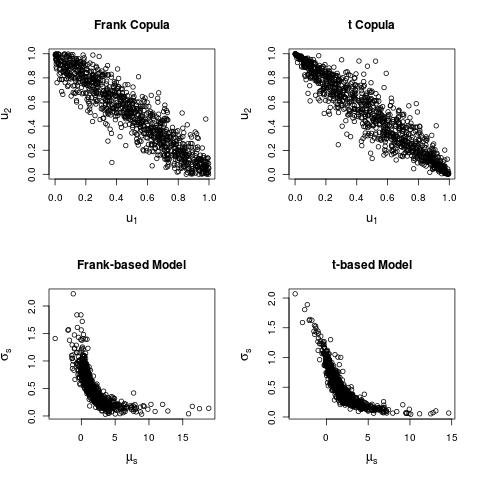
\includegraphics[width=0.9\textwidth]{sdt_copulas}
\caption{The top two panels show samples from a Frank copula and a t copula. Bivariate distributions resulting from applying a t and a gamma transformation to copula samples are in the bottom panel. Parameter settings: $\theta_F = -15, \theta_t = -0.95, \omega = 2, \nu = 3, \lambda = 1.5, \alpha = 3, \beta = 6$. Parameters result in approximately the same Kendall's measure of correlation.}
\label{fig:copmodels}
\end{figure}
% 
  
An alternative to a Frank copula is a t copula 
\begin{equation}
\label{eqn:tcop}
C_t(u_1, u_2) = \int_{-\infty}^{t_{\nu}^{-1}(u_1)}\int_{-\infty}^{t_{\nu}^{-1}(u_2)}\frac{1}{2\pi(1 - \theta_t^2)^{1/2}}\left(1+\frac{x^2-2\theta_txy+y^2}{\nu(1-\theta_t)}\right)^{-(\nu+2)/2}dxdy,
\end{equation}
where $\nu > 0$ is a degrees of freedom, $\theta_t \in [-1, 1]$ is a correlation parameter, $x \in \mathbb{R}$ and $y \in \mathbb{R}$. Note that the t copula is obtained by applying Corollary \ref{thm:copula} by plugging in quantile functions into the bivariate t distribution function, revealing importance of the corollary for deriving new copulas. A sample from a t copula is shown in Figure \ref{fig:copmodels}. The t sample shows that dependence between $u_1$ and $u_2$ has an elliptical contour with extended tails.

By picking Frank and t copulas we can now describe joint variation in $\mu_s$ and $\sigma_s$. To complete defining models of across-trial variation we need two univariate distributions. For $\mu_s$ I will use a non-central t distribution $F_t$ with degrees of freedom $\omega > 0$ and a shape parameter $\lambda \in \mathbb{R}$ that introduces a skew. The support of t covers the real number line, so it satisfies the range requirement for $\mu_s$. As for $\sigma_s$, I will assign a gamma distribution $F_g$, which has support over the positive real numbers just like $\sigma_s$, with a shape $\alpha > 0$ and a scale $\beta > 0$ parameters.

The two copulas can now be combined with the marginal distributions according to Sklar's theorem to give us two distributions of $\mu_s$ and $\sigma_s$. Model $M_1$ takes the form of
\begin{equation}
F_1(\mu_s,\sigma_s \mid \theta_F,\omega,\lambda,\alpha,\beta) = C_F(F_t^{-1}(u_1 \mid \omega,\lambda), F_g^{-1}(u_2 \mid \alpha,\beta) \mid \theta_F),
\end{equation}
and model $M_2$ is
\begin{equation}
F_2(\mu_s,\sigma_s \mid \theta_t,\nu,\omega, \lambda,\alpha,\beta) = C_t(F_t^{-1}(u_1 \mid \omega,\lambda), F_g^{-1}(u_2 \mid \alpha,\beta) \mid \theta_t, \nu).
\end{equation}
Samples from $M_1$ and $M_2$ are in the Figure \ref{fig:copmodels}. $M_1$, on the bottom left, induces a negative, monotonically decreasing relation that shows smooth co-variation between $\mu_s$ and $\sigma_s$. To the right of $M_1$, $M_2$ also induces a negative correlation, but has an abrupt shift in the ``slope'' after a certain $\mu_s$ is reached, suggesting two different states a representation may occupy. Overall, Frank and t copulas result in two bivariate distributions of the signal representation properties that have a noise suppressing feature. 

Using the two models we could examine effects of correlated parameters on hits and false alarms. Before showing how to integrate the copula-based distributions with the bivariate binomial mass function, I will present another useful corollary of Sklar's theorem. 
%
\begin{cors}
\label{thm:coppdf}
For a differentiable p--dimensional distribution function with
continuous quantile functions $F_1^{-1},
F_2^{-1}, \dots, F_p^{-1}$, the probability density function
%
\begin{eqnarray}
f(x_1,x_2, \dots, x_p) & = &
\frac{\partial^p F(x_1, x_2, \dots, x_p)}{\partial x_1 \partial x_2 \cdots \partial x_p} \nonumber \\ 
 & = & \frac{\partial^p C(F_1(x_1), F_2(x_2), \dots, F_p(x_p))}{\partial x_1 \partial x_2 \cdots \partial x_p} \nonumber \\
 & = & c(F_1(x_1), F_2(x_2), \dots, F_p(x_p))\prod_{i = 1}^p f(x_i),
\end{eqnarray}
where $c(F_1(x_1), F_2(x_2), \dots, F_p(x_p))$ is a probability density of a copula, and $f(x_i)$ are probability densities of each dimension.
\end{cors}
%
One important consequence of Corollary \ref{thm:coppdf} is that we can derive a copula density by dividing the joint density by the product of marginal densities, revealing again that a copula is the factor that adds dependence between random variables. From the practical side, the implication is that we can define a new multivariate distribution by going directly to the probability density functions. This becomes useful when marginal distribution functions have no analytical form (e.g. t random variable). 

Going back to the signal detection example, we can now obtain a functional form for hits and false alarms under parameter variability. Let's concentrate on $M_2$ as a model of $\mu_s$ and $\sigma_s$. By Corollary \ref{thm:coppdf}, a density form of $M_2$ is a product of a t copula density $c$ with a noncentral t density $f_t$ and a gamma density $f_g$, so
\begin{eqnarray}
f(\mu_s,\sigma_s \mid \theta_t, \omega, \lambda, \nu, \alpha, \beta) = c(F_t(\mu_s \mid \lambda, \nu), F_g(\sigma_s \mid \alpha, \beta) \mid \lambda) \times \nonumber \\
f_t(\mu_s \mid \lambda, \nu)f_g(\sigma_s \mid \alpha, \beta).
\end{eqnarray}
Then, in an experiment where we observe $N_s$ signal trials and $N_{fa}$ trials, with assumption of variable $\mu_s$ and $\sigma_s$ according to $M_2$,
the probability mass function for hits and false alarms is
\begin{eqnarray}
\int_{-\infty}^{\infty}\int_0^{\infty}p(y_h \mid \mu_s, \sigma_s, \tau, N_s)p(y_{fa} \mid \tau, N_{fa})f(\mu_s,\sigma_s \mid \theta_t, \omega, \lambda, \nu, \alpha, \beta)d\mu_sd\sigma_s = \nonumber \\
p(y_h \mid \theta_t, \omega, \lambda, \nu, \alpha, \beta, \tau, N_s)p(y_{fa} \mid \tau, N_{fa}).
\end{eqnarray}

With two alternative models of hits and false alarms at hand, we could now fit real data and test for the assumption of a dynamic representation of signals. It would be of particular interest to obtain copula parameters. A visual summary of the best model could be captured by a graph of a copula to reveal what sort of joint variation is consistent with data. 

Estimated copula parameters also provide a numerical summary of inference, but they may be more difficult to interpret and it would be beneficial to map them onto commonly used scalar measures of dependence. Due to Sklar's result, it turns out that copulas provide a natural way for deriving several important measures of dependence between random variables, regardless of univariate marginals. 

The most likely attempt at connecting copula parameters to common measures of dependence may be through Pearson's scalar measure of linear dependence 
\begin{equation}
\psi_P = \frac{\mathrm{Cov}\left[x, y\right]}{\sqrt{\mathrm{Var}\left[x\right]\mathrm{Var}\left[y\right]}},
\end{equation}
but it turns out not to work.
It is appropriate when samples come from a normal or a t distribution \citep{CasBer2002}. However, Pearson's coefficient cannot be rewritten strictly in terms of a copula, and when the joint distribution is t, the coefficient may be undefined because moments may not be defined at lower degrees of freedom. Another downside is that marginal distributions of x and y have influence on the Pearson's measure through the $\mathrm{Var}$ operator, revealing that it is partially influenced by marginal variation.

As an alternative, Kendall's  coefficient, which
measures the amount of monotonic dependence between two random variables,
can be defined strictly in terms of a bivariate copula \citep{Joe1997,Nel2007}.  For a bivariate random vector $(x, y)^T$ drawn from a copula $C(\cdot)$ (with probability density $c(\cdot)$), the Kendall's coefficient equals
\begin{eqnarray}
\lefteqn{4 \iint_{[0,1]^2}C(u,v)c(u,v)dudv - 1} \nonumber \\ 
& = & 4 \mathrm{E}\left[C(u,v)\right] - 1.
\end{eqnarray}
The advantages of Kendall's coefficent is that it extends to monotonic relations between variables, does not depend on marginal distributions and provides a familiar scale for comparing different copula-based models. For example, in the generalized signal detection case, with a model of hits and false alarms based on a t copula, Kendall's coefficient is
\begin{equation}
\label{kend_dep}
\rho_k = \frac{2}{\pi}\arcsin(\theta_t),
\end{equation}
which is readily computable.

In addition to general dependence, the tail dependence is a second scalar measure that can help to quantitatively characterize relations between random variables in a simple form. This quantity considers dependence imposed by a copula only in the lower-left or upper-right quadrants. The tail dependence is defined as an asymptotic probability that $x_2$ exceeds some quantile $q$ given that $x_1$ exceeds $q$, corresponding to co-occurence of variables in the extremes. The  lower-left tail dependence
\begin{equation}
\lambda_L = \lim_{q \to 0}P\left(x_2 \leq F_2^{-1}(q) \mid x_1 \leq F_1^{-1}(q)\right), 
\end{equation}
and the upper-right tail dependence
\begin{equation}
\lambda_R = \lim_{q \to 1}P\left(x_2 > F_2^{-1}(q) \mid x_1 > F_1^{-1}(q)\right).
\end{equation}
Similar to the Kendall's coefficient, the tail dependence can be defined  strictly in terms of a copula $C(\cdot)$. For the lower-left tail, the dependence 
\begin{equation}
\lambda_L = \lim_{q \to 0^+}\frac{C(q, q)}{q},
\end{equation}
and for the upper-right tail
\begin{equation}
\lambda_U = \lim_{q \to 1^-}\frac{1 - 2q + C(q, q)}{q}.
\end{equation}

For example, take the t and Frank copulas used in generalizing the standard signal detection model, the former has tail dependence and the later has no tail dependence. Tail dependence can be seen in Figure \ref{fig:copmodels}, especially after applying the quantile transformations, which result in rounded tails for the Frank-based model and sharp tails in the t-based model. In this context, tail dependence could correspond to a representational processes where noise remains tightly bound to a minimal value at high magnitudes of signal.

In conclusion, copulas provide a useful and powerful way of defining new multivariate distributions with various patterns of dependencies which can be easily summarized with scalar quantities. The signal detection model generalization examined in this section serves as a direct example of how models of simple choice behavior can be generalized to have dependent across-trial variation in their parameters. In the next section, I apply the copula-based approach to propose two multivariate distributions for parameter variation that can be used to generalize the Ratcliff diffusion model.

%%%%%%%%%%%%%%%%%%%%%%%%%%%%%%%%%%%%%%%%%%
\section{Proposed Generalizations}
%%%%%%%%%%%%%%%%%%%%%%%%%%%%%%%%%%%%%%%%%%

Recall that one of the questions motivating this thesis is developing a model of across-trial variability of parameters of a sequential sampling model. Going with the descriptive approach I will present two new multivariate distributions that we can use to generalize the Ratcliff diffusion model. Resulting mixture models will set up the stage for answering the other questions guiding this thesis.

I assume the Wiener process as a description of the decision process underlying simple choice behavior. To avoid inconvenient domain of the starting point, I will work
with bias parameterization of the Wiener process where $\beta = \zeta \backslash \alpha$, instead of $\zeta$, fixes the starting value of accumulation. Three parameters are assumed to vary across trials: drift rate, bias and non-decision time. Our problem is to find a couple of multivariate densities that describe behavior of the three parameters, each of which falls on a different scale and has a different univariate distribution. Sklar's theorem tells us that in order to describe joint variation of the three parameters we need a copula and marginal probability density functions for each dimension.
    
I start with copulas. When searching for copulas I concentrated on families that were flexible and computationally tractable. I interpret flexibility as
the ability of a copula to produce different correlations
for each pair of parameters ranging from full negative to full positive dependence.
Basically, we need copulas that can encode as many different types of
correlation structures as possible. Within the set of existing copulas, many
copulas, regardless of the dimension, are governed by a single
parameter that induces a particular kind of dependence
\citep{Joe1997,Nel2007}. For example, Archimedean copulas are
controlled by a single parameter and encode the same lower tail,
upper tail, or all-positive dependence for all
pairs of variables. Frank copula presented in the previous section is an example. Archimedean and other restricted copulas are inadequate because there is no prior information
available about the correlation structure of parameters, so it is sensible to start modeling with most flexible copulas.
    
The elliptical class of
copulas satisfies the flexibility and tractability criterion. Elliptical copulas arise from n-dimensional elliptical distributions that can be defined in terms of their probability density
\begin{equation}
f(\bf{x} \mid \boldsymbol{\mu}, \boldsymbol{\Sigma}) = |\boldsymbol{\Sigma}|^{-1}g \left((x - \boldsymbol{\mu})^T\boldsymbol{\Sigma}^{-1}(x - \boldsymbol{\mu})\right),
\end{equation}
where $|\cdot|$ is a determinant, $g$ is a nonnegative function on positive real numbers, $\boldsymbol{\mu} \in \mathbb{R}$ is a location parameter, and $\boldsymbol{\Sigma}$ is a positive definite scale parameter \citep{Joe1997,Nel2007}. The term ``elliptical'' refers to the quadratic form (argument of $g(\cdot)$) that causes iso-density contours to take the shape of a hyperellipsoid.
Specifically, I propose
using normal and t copulas from the elliptical class. 

Lets consider a normal copula first. Taking the three dimensional standard normal distribution function  $\Phi_3(\bf{x} \mid \bf{P_n})$, $\bf{x} \in \mathbb{R}^3$, with a positive definite correlation matrix 
%
\begin{equation}
\boldsymbol{P}_n = \left[ \begin{array}{ccc}
1 & \rho_{1, 2} & \rho_{1, 3} \\
\rho_{1, 2} & 1 & \rho_{2, 3} \\
\rho_{1, 3} & \rho_{2, 3} & 1
\end{array}
\right], \nonumber
\end{equation}
%
and the standard normal quantile function $\Phi_i^{-1}(u_i)$, $u_i \in [0, 1]$, Corollary \ref{thm:copula} (Equation \ref{eqn:copula}) implies that the normal copula 
%
\begin{equation}
C_n (\boldsymbol{u} \mid \boldsymbol{P}_n) 
  = \Phi_3(\Phi_1^{-1}(u_1),
               \Phi_2^{-1}(u_2),
               \Phi_3^{-1}(u_3) \mid \boldsymbol{P}_n).
\end{equation}
%
Thus, the normal copula equals
%
\begin{eqnarray}
\int_{-\infty}^{\Phi^{-1}(u_1)} \int_{-\infty}^{\Phi^{-1}(u_2)} 
        \int_{-\infty}^{\Phi^{-1}(u_3)} 
        |(2\pi\boldsymbol{P}_n)|^{-1 / 2}\exp\left(-\frac{1}{2}\boldsymbol{x}^T
\bf{P}_n \bf{x}\right)d\bf{x},
\end{eqnarray}
%
where $\boldsymbol{x} \in \mathbb{R}^3$.
By Sklar's theorem, coupling the normal copula $C_n (\boldsymbol{u} \mid \boldsymbol{P}_n)$ with three normal
marginals $F_i(x_i)$ will result in the
multivariate normal distribution function $C(F_1(x_1), F_2(x_2), F_3(x_3) \mid \boldsymbol{P}_n)$, but substituting some other univariate marginals $G_i(x_i)$ into
the normal copula will result in a novel probability distribution $C_n(G_1(x_1), G_2(x_2), G_3(x_3) \mid \boldsymbol{P}_n)$.

$t$ is the second copula that I propose to use. Derivation of a $t$ copula is also a consequence of applying Corollary \ref{thm:copula}. Given a 3-dimensional t cumulative distribution function $T_3(\cdot)$ and a t quantile function $t_i^{-1}(u_i)$, the t copula 
%
\begin{eqnarray}
C_t(\boldsymbol{u} \mid \boldsymbol{P}_t,\omega) = T_3(t_1^{-1}(u_1 \mid \omega),
           t_2^{-1}(u_2 \mid \omega),
           t_3^{-1}(u_3 \mid \omega) \mid \boldsymbol{P}_t), 
\end{eqnarray}
where $\boldsymbol{P}_t$ is a positive definite correlation matrix like in the normal copula, and $\omega > 0$ is a degrees of freedom parameter.
Definitions of $T_3(\cdot)$ and $t_i^{-1}(\cdot)$ imply that the t copula equals
\begin{eqnarray}
\int_{-\infty}^{t^{-1}(u_1 \mid \omega)}
       \int_{-\infty}^{t^{-1}(u_2 \mid \omega)}
       \int_{-\infty}^{t^{-1}(u_3 \mid \omega)}
       \mathcal{G} \left([\omega+3] / 2\right) / \left[\mathcal{G}(2\omega)\sqrt{|\pi\omega\boldsymbol{P}_t|}\right]  \nonumber \\  
\times \left( 1 + \boldsymbol{x}^T\boldsymbol{P}_t^{-1 / 2}\boldsymbol{x} /
{\omega} \right)^{(\omega + 3) / 2}d\boldsymbol{x},
\end{eqnarray}
%
where $\mathcal{G}(\cdot)$ is a univariate gamma function and $\boldsymbol{x} \in \mathbb{R}^3$.
Unlike the normal copula, the t copula has a degrees of freedom parameter $\omega$ that results in heavier tails. The parameter $\omega$ introduces
additional flexibility that controls probability of
extreme values in the tails, resulting in positive tail dependence, and combinations of parameters
orthogonal to the correlation structure. 

As an example of orthogonality, suppose correlation
between two parameters is positive, it is unlikely that we
might observe a pair of values where one point has high magnitude and
the second point has low magnitude. However, the occurence of
such rare events is predicted for finite values of
$\omega$ with considerably higher probability than for the normal copula. When $\omega \to \infty$, the t copula
converges to the normal copula \citep{Joe1997}. Thus, a model of parameter variation based on the t copula is a further generalization of the normal copula that allows modeling correlations between processing components that sometimes take unusual combinations or extreme values in the tails.

To complete definitions of two models of parameters, Sklar's theorem
requires that we specify marginal distributions for each
parameter. Since I am modeling parameters in a descriptive manner and variation of parameters is unobservable, I limited my search to univariate distributions that exhibit flexible shapes to enable good approximations of the true shape. In contrast, if I were following a mechanistic approach, I would want to produce marginal variation that agrees with observations and disallow all other distributional shapes.

For the drift rate $\delta$, in line with the
Ratcliff model, I will assume a normal distribution. I will
replace Ratcliff's continuous uniform assumption for the non-decision
parameter $\tau^{nd}$ with a truncated normal distribution,
and place a beta distribution on bias parameter
$\beta$. The univariate marginals for the three parameters are therefore
%
\begin{eqnarray}
\delta & \sim & \mathcal{N}(\nu, \eta^2), \nonumber \\
\beta & \sim & \mathcal{B}(\lambda, \gamma), \text{and} \nonumber \\
\tau^{nd} & \sim & \mathcal{TN}(\chi,\phi^2,a,b),
\end{eqnarray}
 where $\lambda > 0$ and $\gamma > 0$ are shape parameters, $\chi \geq a$ is a location parameter, $\phi > 0$ is a scale parameter, $a$ and $b$ are truncation points such that $0 \leq a < b < \infty$. 
 
Now we can combine specified copulas and univariate marginals. Applying Sklar's theorem leads to
$i = 1, 2$ new multivariate distributions of the form
%
\begin{equation}
F_i(\delta,\beta,\tau^{nd}) = C_i(F_1(\delta),F_2(\beta),F_3(\tau^{nd})),
\end{equation}
%
from which, by Corollary \ref{thm:coppdf}, we can obtain probability densities by 
%
\begin{equation}
f_i(\delta,\beta,\tau^{nd}) 
   = c_i(F_1(\delta),
         F_2(\beta),
         F_3(\tau^{nd}))
         f_1(\delta),f_2(\beta),f_3(\tau^{nd}).
\end{equation}
 
The copula density and marginal densities have known analytic
expressions
\citep{Nel2007,CasBer2002,JohKot1994,JohKot1995}.  Direct application
of the Sklar's theorem ensures that both models of parameter
variability are valid distributions or densities. 
This completes generalization of the Ratcliff
diffusion model of simple decisions. We can now proceed to study implications of the proposed model set.

%%%%%%%%%%%%%%%%%%%%%%%%%%%%%%%%%%%%%%%%%%%%%%%%%%%%%%%%%%%%%%%%
\chapter{Proposed studies}
%%%%%%%%%%%%%%%%%%%%%%%%%%%%%%%%%%%%%%%%%%%%%%%%%%%%%%%%%%%%%%%%

With models of behavior defined, I can now outline two studies designed to answer the remaining questions. Recall that I proposed to compare predictions of the models and analyze the nature of the correlation structure consistent with the benchmark data. In study A, I plan to explore effects of parameter correlations on models' predictions under an experimental design similar to \citet{RatRou1998}. The objective is to compare predictions of mean sample paths, and commonly found features of response and response times that follow from their joint densities.

After, study B will outline application of the proposed models to the benchmark dataset. Posterior densities of parameters and predictions will be obtained with MCMC. The goals are to infer direction and plausible values of correlation parameters, compare quality of predictions of fitted models for important features of behavioral data and determine the effect of adding a correlation structure on adjusted measure of overall predictive accuracy.

%%%%%%%%%%%%%%%%%%%%%%%%%%%%%%%%%%%%%%%%%%%%%%%%%%%%%%%%%
\section{Study A: Comparison of Models' Predictions}
%%%%%%%%%%%%%%%%%%%%%%%%%%%%%%%%%%%%%%%%%%%%%%%%%%%%%%%%%

Study A will examine predictions of the standard Ratcliff diffusion models and its generalizations proposed above. I will first outline exactly what predictions I propose to use for model comparison. It turns out that all these predictions require solutions of analytically intractable integration problems, so along with predictions I will describe methods of approximation appropriate for each problem. Then, I will describe the experimental design and values of free parameters under which predictions will be calculated. Finally, I will describe graphical and quantitative means of comparing the three models and discuss limitations of this study.

%%%%%%%%%%%%%%%%%%%%%%%%%%%%%%%%%%%
\subsection{Mean Sample Paths}
%%%%%%%%%%%%%%%%%%%%%%%%%%%%%%%%%%%

One prediction of the three decision models that can provide insight into effects of correlations among parameters of a Ratcliff diffusion model include mean sample paths. Mean sample path, $\mathrm{E}[x(t)]$, is an unconditional mean of a stochastic process at each time point. For the Wiener process with no boundaries, it is available in analytical form and is equivalent to a line $\delta t + \zeta$, where the drift rate $\delta$ is the slope and the starting point $\zeta$ is the y-intercept. However, for a Wiener process with absorbing boundaries, as required for the decision process model, the dynamics changes in a non-trivial way and the mean sample path is not available in explicit form. The calculation is further complicated by variable parameters.

However, we can still obtain predictions by realizing that the mean sample path is an integral problem at each time point. Lets consider the value of the sample path of a bounded Wiener process with fixed parameters at some time t. Then, the mean sample path
\begin{equation}
\mathrm{E}[x(t)] = \int_{\mathcal{S}}x(t)f(x(t))dx(t),
\end{equation}
where $\mathcal{S}$ is the bounded state space and $f(x(t))$ is the marginal density. Since $f(x(t))$ is unavailable, we cannot use numerical integration. However, the problem could be solved if we could sample from $f(x(t))$ and then use a Monte Carlo estimator to approximate the sample path at time t. 

The Monte Carlo estimator appropriate to this problem is a consequence of a law of large numbers for independent and identically distributed random variables \citep{CasBer2002}. For a random sample $x_1(t), x_2(t), \ldots x_N(t)$ $\sim$ $f(x(t))$, with expected value $\mathrm{E}[x(t)] < \infty$,  
\begin{equation}
\lim_{N \to \infty}\frac{1}{N}\sum_{i=1}^N x_i(t) = \mathrm{E}[x(t)].
\end{equation}
When N is fine, the left hand side, or the Monte Carlo estimator, approximates the expected value.

To obtain a Monte Carlo estimate of the mean sample path we need samples from the marginal density over a grid of time points. One way to obtain such samples is to simulate the Wiener process until it hits an absorbing boundary. Each simulated path provides a draw from the marginal density at each time point of the grid. Since sample paths are generated independently, values of the process at time $t$ make an independent sample. Hence, assumptions for the Monte Carlo estimator hold for each time point. The issue, however, is how to average the sample paths given that they will have different lengths. 

One way to resolve the length issue is to align paths either on the initial time or the absorption time, and average paths along the length of the shortest path. This way one can estimate either the initial or final part of the mean sample path. I propose aligning at the absorption time because that is where dynamics is different from the unbounded process and effects of parameter correlations will be most visible as they buildup over the time course of a decision.

The above considerations were made under the assumption of fixed parameters, but variable parameters pose no difficulty. The Ratcliff diffusion model and its generalizations assign some multivariate density over the parameter. To obtain a mean sample path we would just average a mean sample path for fixed parameters with respect to the parameter density. Since it is just another layer of integration, the Monte Carlo method will automatically calculate it if we simulate in a hierarchical manner.

In a hierarchical simulation, we need to incorporate variability in parameters. For the decision model $i = 1, 2, 3$, a hierarchical procedure to obtain estimates of the mean sample paths will involve
\begin{enumerate}
\item Simulate N draws of $(\nu, \zeta) \sim f(\nu, \zeta \mid \nu, \eta^2, \lambda, \gamma)$
\item Simulate N sample paths $x(t \mid \nu, \zeta, \alpha)$
\item Align and average sample paths from 2 along the shortest path.
\end{enumerate}
The procedure for estimating mean sample paths is computationally simple and fast. Simulation in Step 1 can obtained with base and copula packages of R statistical environment \citep{HofKoj2013,R2014}. For step 2, I have a custom R program for a random walk approximation of the Wiener process \citep{TueMar2001}.   

To conclude, understanding of how correlated parameters affect the time course of a decision process can be revealed by comparing mean sample paths of the standard to generalized Ratcliff diffusion models. The calculation of $\mathrm{E}[x(t)]$ is very difficult, but we can be obtain it by simulating the bounded Wiener process with variable parameters and then averaging sample paths. From examining mean sample paths we can move to studying effects of correlated parameters on response times and responses, which arise from sample paths being absorbed at some time and some boundary.   

%%%%%%%%%%%%%%%%%%%%%%%%%%%%%%%%%%%%%%%%%%%%%%
\subsection{Response times and Responses}
%%%%%%%%%%%%%%%%%%%%%%%%%%%%%%%%%%%%%%%%%%%%%%

While studying mean sample paths under correlated parameters will suggest how the decision process changes, examining the joint density of response times and responses should show how behavior changes. Recall that the joint density is a mixture model averaged with respect to variability in parameters, such that for model $i = 1, 2, 3$
\begin{equation}
f_i(t^{rt}, r \mid \boldsymbol{\theta}_i) = \int_A f(t^{rt},r \mid \alpha, \delta, \zeta)f_i(\delta, \zeta \mid \boldsymbol{\theta}_i)dA, 
\end{equation}
where $\boldsymbol{\theta}_i$ will reflect the correlation structure and other parameters defined as above. 

For a fixed correlation structure, the joint density of behavior contains all the predictions of interest. We could look at its shape, which consists of two density components, one for each response. Or examine summary features like the vector mean of response time and response, and their covariance matrix. However, a more popular approach in examining simple choice behavior requires examining response probabilities of each choice and response time density functions conditioned on choice \citep{Vic1979,Luc1986}, both of which follow from the joint density. I will adopt the standard approach because it matches behavioral heterogeneity of different choices  and provides a systematic way of examining effects of a correlation structure. 

To determine effects of a correlation structure I propose to examine shapes of conditional densities and their varies summary features. We can obtain conditional densities by normalizing the joint density with a probability of response. For response r and model i, conditional density of response time is
\begin{equation}
f_i(t^{rt} \mid r, \boldsymbol{\theta}_i) = f_i(t^{rt}, r \mid \boldsymbol{\theta}_i) / P\{r = c\},
\end{equation}
where $c \in \{0, 1\}$ is a choice.
One feature of conditional densities worth examining is their overall shape. Observed shapes are positively skewed and change in characteristic ways across experimental conditions. The correlation structure should have effects on the shape and provide a qualitative way of comparing the models.

In contrast to qualitative comparisons, we can also calculate summary features of each conditional density that quantitatively characterize their shapes. To provide an informative account of effects of correlated parameters it is necessary to capture location, scale, shape and the corresponding response probabilities (normalizing constants) of each conditional density of response time. For location I will use the expected value as a measure of location, $\mathrm{E}_i[t^{rt} \mid r] = \mu_{r,i}$, 
and standard deviation as a measure of scale, $\sqrt{\mathrm{E}_i[(t^{rt} - \mu_{r,i})^2 \mid r]}$. The shape is a complex concept with many components, but here I propose to use skew,
\begin{equation}
\mathrm{Skew}_i[t^{rt} \mid r] = \frac{\mathrm{E}_i\left[(t^{rt} - \mu_{r,i})^3 \mid r \right]}{\mathrm{E}_i[(t^{rt} - \mu_{r,i})^2 \mid r]^{3/2}},
\end{equation}
and excess kurtosis,
\begin{equation}
\mathrm{Kurtosis}_i[t^{rt} \mid r] = \frac{\mathrm{E}_i\left[(t^{rt} - \mu_{r,i})^4 \mid r \right]}{\mathrm{E}_i[(t^{rt} - \mu_{r,i})^2 \mid r]^2} - 3,
\end{equation}
as two measures that can characterize shape. Data shows consistently positive skew of response times, which can be measured by skew, and excess kurtosis can capture increase in the amount of extreme response times relative to what can be expected under a normal density. Lastly, the probability of hitting the upper boundary
%
\begin{eqnarray}
P_i\{r = 1\} = \nonumber \\
\int_{\delta \times \beta} \left[\exp\left(\frac{-2\delta\alpha\beta}{\sigma^2}\right)-1\right]/
                \left[\exp\left(\frac{-2\delta \alpha}{\sigma^2}\right)-1\right]f_i(\delta, \beta \mid \boldsymbol{\theta}_i)d\delta d\beta,
\end{eqnarray}
%
where the probability of hitting the lower boundary is a complementary probability.

Notice that getting conditional densities and calculating all the summary features again requires integration. Similar to the problem of finding mean sample paths, the integrals are intractable, but in this case the probability density is known and computable \citep{Tue2004,NavFus2009}. Instead of using a Monte Carlo estimate, we can use deterministic approximation methods based on quadrature. Similar to the Monte Carlo estimator, quadrature methods approximate an integral with a weighted average, such that
\begin{equation}
\int_{\mathcal{X}}g(x)dx \approx \sum_{i=1}^N w_i g(x_i),
\end{equation}
but weights $w_i$ can be other than $1/n$ and nodes $x_i$ are set deterministically.

To obtain behavioral predictions, I propose using a globally adaptive integration algorithm  \citep{GenMal1980,BerJar1991}. It is highly efficient for 2 and 3 dimensional integrals, and precision can be guaranteed deterministically. An optimized code has been implemented in C and can be called using R package cubuture \citep{JohNar2013}.

With predictions worth exploring outlined, we now need to identify a task and experimental conditions under which predictions for decision process and behavior can be compared. In the next section, I outline how to obtain predictions for a brightness discrimination task used by \citet{RatRou1998}.

%%%%%%%%%%%%%%%%%%%%%%%%%%%%%%%%%%%
\subsection{Parameter Settings}
%%%%%%%%%%%%%%%%%%%%%%%%%%%%%%%%%%%
By now, predictions of interest and methods for their calculations have been specified. Next, I lay out experimental conditions under which predictions will be obtained. I follow the principle that predictions should be obtained for a particular task under realistic experimental conditions. Since models will later be fit to the benchmark dataset it is most natural to expore predictions for the underlying brightness discrimination task. 

Recall that the \citet{RatRou1998} benchmark dataset was generated by a two-choice free response perceptual task under 33 brightness levels and speed-accuracy instructions. They had 3 subjects, but they showed similar behavior and parameters, so I will concentrate on a single individual. To calculate predictions we need parameter values that reflect experimental manipulations experienced by the individual. One approach could be to eyeball parameters representing effects of manipulations from a range of plausible values that were recovered over many experiments \citep{MatWag2009}. In contrast, since it is a benchmark dataset, there are parameter estimates for the Ratcliff diffusion model available, both Bayesian and non-Bayesian \citep{RatRou1998,VanTue2011}. I propose using the means of posterior densities from \citet{VanTue2011} to obtain predictions.

Bayesian modeling done by \citet{VanTue2011} took certain assumptions about how experimental manipulations influence parameters. In their best fitting model, authors assumed that brightness level affects only mean drift rate and speed-accuracy instructions affect drift rate, boundaries and starting position, with other parameters being constant across the experimental sessions. I will calculate predictions under these assumptions, too.

For the drift rates, \citet{VanTue2011} provided a descriptive front-end model of how rate of evidence accumulation arises from brightness levels under particular instructions. The formal relation is described by the Weibull function. For instruction $i = 1, 2$ and brightness level $j = 1, 2, \ldots, 11$, I assume mean drift rate regresses on brightness level through a sigmoidal-shaped Weibull function 
%
\begin{equation}
\nu_{i,j} = \nu_{i}^{lo}+\left(\nu_{i}^{hi}-\nu_{i}^{lo}\right)   \left(1 - \operatorname{exp} \left( [-p_{j}/\nu_{i}^{sc}]^{\nu_{i}^{sh}}
\right) \right),
\end{equation}
%
where $\nu_{i,j}$ is the drift rate, $p_{j}$ is the brightness proportion, $\nu_{i}^{lo}$ is the lower asymptote, $\nu_{i}^{up}$ is the upper asymptote, $\nu_{i}^{sc}$ is the scale parameter and $\nu_{i}^{sh}$ is the shape parameter. The estimates of Weibull parameters taken from \citet{VanTue2011} are in Table \ref{tab:weibull}.

\begin{table}[H]
\centering
\begin{tabular}{|l*{4}{|c}|r|}
\hline
Instruction & $\nu_{lo}$ & $\nu_{hi}$ & $\nu_{sh}$ & $\nu_{sc}$ \\ \hline
Accuracy & -0.352 & 0.329 & 4.413 & 0.526 \\ \hline
Speed 	 & -0.565 & 0.511 & 5.227 & 0.521 \\ \hline
\end{tabular}
\caption{\label{tab:weibull} \textbf{Weibull function parameters}}
\end{table}

The Weibull function provides a parsimonious way of connecting 66 experimental conditions to drift rates via 8 parameters. However, for obtaining predictions I do not need all 66 conditions. Based on previous fits to the benchmark dataset \citep{RatRou1998,VanTue2011}, and more commonly observed in psychophysical investigations \citep{Vic1979,Rat2014}, drifts and discriminability performance level off for extremely bright or dark stimuli. The drift rates change sigmoidally as a function of brightness level and are most informative for proportions from 0.2 to 0.8. Hence, I can use points in that range that were also used in the benchmark experiment to set drift rates. More specifically, I propose to use 11 white-to-black pixel proportions, \{0.188, 0.250, 0.313, 0.375, 0.438, 0.500, 0.563, 0.625, 0.688, 0.750, 0.813\}, which will give a sufficient number of points to capture the shape of predicted curves.

The other non-correlation parameters are listed in Table \ref{tab:noncor}. The values for thresholds $\alpha_i$ and drift rate standard deviation $\eta$ are taken directly from \citet{VanTue2011}. Mean bias $\lambda_i$ and standard deviation of bias $\gamma$ are transformation of end point estimates because I assumed a beta density whereas \citet{VanTue2011} assumed a continous uniform density. Similarly, \citet{VanTue2011} assigned a normal density to the non-decision parameter whereas I assigned a normal truncated at 0, so their estimates of mean and standard deviation are now location and scale parameters of the truncated normal.

\begin{table}[H]
\centering
\begin{tabular}{|l*{6}{|c}|r|}
\hline
Instruction & $\alpha$ & $\eta$ & $\lambda$ & $\gamma$ & $\chi$ & $\phi$ \\ \hline
Accuracy & 0.221 & 0.127 & 0.464 & 0.065 & 0.279 & 0.041 \\ \hline
Speed 	 & 0.050 & 0.127 & 0.464 & 0.008 & 0.279 & 0.041 \\ \hline
\end{tabular}
\caption{\label{tab:noncor} \textbf{Non-correlation parameters}}
\end{table}

The remaining parameters are the degrees of freedom for the t copula and correlation parameters that characterize generalized diffusion models. I will fix the degrees of freedom $\omega$ to 5, which would lead to t copula having all its moments and being maximally different from the normal copula. $\omega$ will be assumed to be the same throughout the experiment. 

Lastly, I propose to examine three correlation structures with low, medium and high levels of correlation between parameters, which will also stay the same throughout the experiment. The patterns are in Table \ref{tab:corr}. The structures reflect a few of many possible correlation patterns that could exist
under typical experimental conditions. The selected patterns can be interpreted to represent different processing situations. For example, based on the pattern of signs, sets 1 - 3 can be interpreted as a tendency of decision bias $\beta$ and evidence $\delta$ agreeing on the best response while the non-decision $\tau^{nd}$ reflectes motor bias towards the other response. Thinking through the behavioral consequences of other correlation structures, similar interpretations can be proposed, but these are only suggestive and were used to select the 3 proposed correlation patterns out of the infinitely many possibilities without any theoretical commitment.
%
\begin{table}[H]
\centering
\begin{tabular}{|l|c|c|r|}
\hline
Set & $\rho_{\delta,\beta}$ & $\rho_{\delta,\tau^{nd}}$ & $\rho_{\beta,\tau^{nd}}$ \\ \hline
1 & 0.15 & -0.15 & -0.15 \\ \hline
2 & 0.50 & -0.50 & -0.50 \\ \hline
3 & 0.85 & -0.85 & -0.85 \\ \hline
4 & -0.15 & 0.15 & 0.15 \\ \hline
5 & -0.50 & 0.50 & 0.50 \\ \hline
6 & -0.85 & 0.85 & 0.85 \\ \hline
7 & -0.15 & -0.15 & 0.15 \\ \hline
8 & -0.50 & -0.50 & 0.50 \\ \hline
9 & -0.85 & -0.85 & 0.85 \\ \hline
\end{tabular}
\caption{\label{tab:corr} \textbf{Correlation parameters}}
\end{table}
%

The combination of proposed parameters should lead to interpretable comparisions between the three models. All calculations will be done under the same parameter values for all the non-correlation parameters, and correlation parameters will be the same for the two copula-based models. The only differencees between the models are the copula assumptions. The Ratcliff diffusion model has the independence copula and generalizations have the normal and t copulas. 

More over, the copula-based models will be matched in their Kendall coefficients for each correlation pattern because, as mentioned in the copula section, they both belong to a class of elliptical distributions whose Kendall's coefficient is equal to $2\arcsin(\rho)/\pi$. However, recall that the t copula is nevertheless distinct by having symmetric tail dependence (the asymptotic probability that two random variables are both extreme). For the t copula, the tail dependence is equal to
\begin{equation}
\label{tail_dep}
2t_{\omega}(-\sqrt{\omega + 1}\sqrt{1 - \rho}/\sqrt{1 + \rho}),
\end{equation}
where $t_{\omega}$ is a t cumulative distribution function, $\omega$ is degrees of freedom and $\rho$ is the correlation parameter. The tail dependence is determined by both parameters of a t copula, which gives a more concrete justification for choosing $\omega = 5$ since it ensures that t copula is distinct from a normal copula in its tail dependence. 

In conclusion, the proposed set of parameters is intended to enable unambiguous conclusions about how the three models differ in the predictions based solely on their parameter dependence assumptions. In the next section I will describe several means of organizing predictions to facilitate comparison and establish differences between models.

%%%%%%%%%%%%%%%%%%%%%%%%%%%%%%%%%%%%%%%%%%%%%%
\subsection{Results}
%%%%%%%%%%%%%%%%%%%%%%%%%%%%%%%%%%%%%%%%%%%%%%

How do the three decision models differ in their predictions? We can answer this question in detail graphically and quantitatively. After calculating mean sample paths, conditional densities of response times and their summary features, I will organize them graphically and provide calculations of prediction differences where models diverge the most. 

Trajectories of mean sample paths naturally form a time series. To understand how correlation between $\zeta$ and $\delta$ affects shapes of samples I will overlay Monte Carlo estimates for the three models for each combination of brightness and instructions. The combination of 22 plots will reveal qualitatively how time course of decision process is shaped by one of 9 correlation structures.

The conditional densities of response times can also be graphically compared to capture effects on the overall shape. Juxtaposing conditional densities in a manner of violin plots will reveal asymmetries between the two choices. The full pattern of variation in the density shape will be examined across combinations of experimental condition and correlation structure.

The shapes of conditional densities can be compared quantitatively using various summary features. For each density, there will be mean, standard devition, skew, curtosis and probability of the corresponding response. I will examine how the summary features vary as a function of brightness level and instruction for each density. From the same prediction data I will also examine simultaneous changes between densities using latency-probability plots that relate mean conditional rection times with probability correct. In addition to the plots, since quantities for all the features will be known, I can also provide precise discrepancies between models for particular conditions.

Overall, the full pattern of graphical and quantitative comparisons of the three models will reveal effects of parameter correlation in detail. The detailed understanding of prediction deviations will enable us to judge which features of data we should pay attention to when evaluating models against the benchmark dataset.

\subsection{Discussion}
Results of model predictions will provide a rich body of data to discuss assumption of correlated parameters. Whatever conclusions may be they will be limited by certain choices underlying this study. The two major sources of limitation are modeling assumptions and response time task assumptions. To examine effects of correlated parameters I propose to use the Ratcliff diffusion model, but other well-established sequential sampling models could be used, too \citep{UshMcc2001,BroHea2008}. Certain features like noisy evidence or perfect integration without inhibition may interact with correlated parameter in a qualitatively different manner from when these assumptions do not hold. Due to sensitivity of decision models to architectural assumptions \citep{Luc1986,RatSmi2004}, conclusions about predictions obtained in this thesis will not be transferable without considerable doubt to other models.

In addition to the accumulation process, taking elliptical copulas to represent correlation structure is also a limitation. In elliptical copulas, while each pair of dimensions can have different signs and magnitudes of correlation, they all have the same linear dependence structure. A more flexible approach is to model dependence of each pair of variables by a different bivariate copula and tie them together into a novel multivariate copula using a tree-like factorization of a multivariate distribution \citep{Cza2010}. If there is some data, such as trial-level Bayes estimates of parameters, that reveals the dependence structure, a custom copula should make the predictions better.

Another major limitation comes from obtaining model predictions under the experimental design and manipulations of the \citet{RatRou1998} study. As discussed in Section \ref{sec:tasks} on page \pageref{sec:tasks}, other response time procedures, like the response signal procedure, could have been used or manipulations of rewards might be added or the number of choices increased. The proposed predictions will be limited to two-choice free response procedure with manipulations of stimulus quality and speed-accuracy instruction.

%%%%%%%%%%%%%%%%%%%%%%%%%%%%%%%%%%%%%%%%%%%%%%%%%%%%%%%%%%
\section{Study B: Benchmark Dataset Analyses}
%%%%%%%%%%%%%%%%%%%%%%%%%%%%%%%%%%%%%%%%%%%%%%%%%%%%%%%%%%

The purpose of Study B is to evaluate the proposed models
against the benchmark behavioral data and estimate the correlation structure. The outline of the study is as follows. First, I will describe outlier pre-processing procedure to deal with extreme response times. After, I will define three hierarchical Bayesian models that will be fit to pre-processed data. A variant of a Metropolis-Hastings algorithm will be defined and convergence diagnostics discussed. Then, I will describe statical analyses that provide an answer to the study questions and discuss limitations of the study.

%%%%%%%%%%%%%%%%%%%%%%%%%%%%%%%%%%%%%%%%%%%%%
\subsection{Outlier Pre-processing}
%%%%%%%%%%%%%%%%%%%%%%%%%%%%%%%%%%%%%%%%%%%%%

An important feature of any dataset involving response times is presence of contaminants. Contaminants are observations arising from processes unrelated to research questions. Some of the recognized types of contaminants are fast guesses, slow guesses and delayed responses
\citep{Rat1993,RatTue2002,VanTue2007,VanTue2008,CraPer2010,
VanTue2011}. Contaminants could arise due to non-compliance with experimental instructions or occasional loss of attention, among other processes. 

To obtain accurate inferences about the process of interest, contaminants need to be either excluded or modeled. The proposed models are complex and initial testing may be more successful without including additional structure required to capture contaminants \cite{RatTue2002,CraPer2010}. Therefore, I will use a set of common procedures to clean up the response time data before fitting the models \citep{Rat1993}.

Since contaminants mixed in with regular response times cannot be identified, the most that is possible to do is to remove outliers. The outlier is defined as an extreme observation relative to the mean of the sample. There are fast and slow outliers that appear in a typical dataset. The fast outliers are usually understood as being equivalent to fast guesses, thus a useful heuristic to detect them is chance performance \citep{RatTue2002}.
  
One way to use chance performance to remove fast outliers is to bin data into continuous intervals. Starting at the lowest multiple of the bin size that includes the fastest response times, we can scan the ordered sequence of observations one interval at a time. For each interval, we calculate accuracy rate. If accuracy is at chance, then responses are fast guesses and they should be excluded. I will define ``at chance'' as an interval between 0.50 and 0.53, taking into account samping error and that probability of exactly chance performance is zero. When accuracy rises above the chance interval, then responses in the bin are due to the process of interest and the lower bound of the bin forms the cut-off for excluding fast responses. 

For the benchmark dataset, I propose using a window of size 50 ms. The individuals and conditions vary a lot, so the method will be more accurate if applied to all the subject by condition combinations as opposed to applying it all the data simultaneously. Preliminary application of the method resulted in a cut-off value of 200 ms for all three subjects. The total number of observations excluded would be 123. 

On the other hand, dealing with extremely long reaction times is different because it includes both slow guesses and delayed responses. In this case, the accuracy signature is not appropriate because delayed responses can be highly accurate since they are generated by the decision process. A practical method to deal with slow outliers is to use a multiple of standard deviations from the mean as a cut-off.

To remove the slow outliers I propose using three standard deviations from the mean as a cut-off. Same as for the fast outliers, I will apply the procedure to all subject by condition combinations to take variability into account. Preliminary application of the cut-offs led to a total removal of 429 observations. Overall, applying proposed procedures would bring the total number of excluded observations to $2\%$ of the full dataset.

%%%%%%%%%%%%%%%%%%%%%%%%%%%%%%%%%%%%
\subsection{Bayesian Models}
%%%%%%%%%%%%%%%%%%%%%%%%%%%%%%%%%%%%

With the data to be modeled established, the remaining task is to describe models to be fitted. The models of performance data I plan to evaluate are hierarchical versions of independent copula diffusion model, the normal
copula diffusion model and the $t$ copula
diffusion model. Multiple variations of these
models could be constructed by making different assumptions about how experimental manipulations, stimulus quality and speed-accuracy instructions, influence cognitive processing. I will rely on results from previous modelling and an EEG study to hypothesize how experimental manipulations affect processing. Finally, while a hierarchy can be defined for all parameters of the model, I will restrict it to parameters of primary interest: parameters that quantify experimental manipulations and correlation parameters. 

I will use the following variables to denote features of the experimental design. The dataset contains $l = 1, 2, 3$ subjects. Each subject received a block-wise instruction $k = 0, 1$, where 0 is speed and 1 is accuracy, combined with a trial-wise brightness level $j = 0, 1, \ldots 32$. For each condition, a subject would have $N_{j,k,l}$ observations. The observations come from a model $M = 1, 2, 3$, referring to independent, normal and t diffusion model, respectively. 

Recall that the joint density of behavior is a mixture of the Wiener first-passage density and a copula-based density. The joint density for model M of a single observation $(t_{i,j,k,l}^{rt}, r_{i,j,k,l})$ conditioned on instruction $k$ and brightness proportion $p_{j}$ is
\begin{equation}
f_M(t_{i,j,k,l}^{rt}, r_{i,j,k,l} \mid p_{j},\alpha_{k, l}, \nu_{j,k,l},\eta_l,\lambda_{k,l},\gamma_{k,l},\chi_{k,l},\phi_{k,l},\rho_l^{\delta,\tau^{er}},\rho_l^{\beta,\delta},\rho_l^{\beta,\tau^{er}}).
\end{equation}
The indeces of parameters reflect individual differences across all parameters. The instructions are assumed to influence thresholds, drift rates and bias in line with previous successful model fits of the benchmark data and similar experiments \citep{RatRou1998,VanTue2007,RatMck2008, Wag2009,VanTue2011}, and also influence nondecision times as indicated by lateralized readiness potential increase under accuracy instruction \citep{RinOsm2004}. The brightness level only influences the drift rates \citep{VosRot2004,RatMck2008,VanTue2011}.

Similar to study A, I will model effect of brightness proportion and instruction on drift rates with a regression function. I assume mean drift rate regresses on brightness proportion through a sigmoidal-shaped Weibull function 
%
\begin{equation}
\nu_{j,k,l} = \nu_{k,l}^{lo}+\left(\nu_{k,l}^{hi}-\nu_{k,l}^{lo}\right)   \left( 
1 - \operatorname{exp} 
\left( 
[-p_{j}/\nu_{k,l}^{sc}]^{\nu_{k,l}^{sh}}
\right)
\right),
\end{equation}
%
\noindent where $\nu_{j,k,l}$ is the drift rate, $s_{j}$ is the brightness level, $\nu_{k,l}^{lo}$ is the lower asymptote, $\nu_{k,l}^{up}$ is the upper asymptote, $\nu_{k,l}^{sc}$ is the scale parameter and $\nu_{k,l}^{sh}$ is the shape parameter. The parameter indices express individual differences and effect of speed/accuracy manipulation on all the parameters \citep{VanTue2011}. This completes specification of model M's data density.

The next part of Bayesian models I specify are priors for all the parameters. All parameters except for correlation parameters and the degrees of freedom are shared by the three models. I will assign the same priors across models to all the shared parameters to maximize similarity. Experience with fitting the Ratcliff model across many tasks and conditions suggests a range of plausible values that can be incorporated through restricting support of priors. I will use recovered parameters from 28 studies reported by \citet{MatWag2009}, but double the reported maximum values to take into account the possibility of yet unobserved rare parameter combinations or imperfect representativeness of tested subjects. The imposed constraints should improve extraction of parameter information from data by reducing posterior variability \citep{GelCar2013}. 

To flexibly impose support constraints while allowing for adaptable distribution of probability mass over the domain, I will use truncated normal priors for the main parameters of interest. The priors for the commonly shared main parameters of interest are
\begin{eqnarray}
% boundary
\alpha_{k,l} \sim \mathcal{TN}(\mu_k^{\alpha},\sigma_k^{\alpha},0.001, 0.786), \nonumber \\
% drifts
\nu_{l}^{lo} \sim \mathcal{TN}(\mu^{\nu^{lo}},\sigma^{\nu^{lo}},-1.172, 0), \nonumber \\
\nu_{l}^{up} \sim \mathcal{TN}(\mu^{\nu^{up}},\sigma^{\nu^{up}},0, 1.172), \nonumber \\
\nu_{l}^{sh} \sim \mathcal{TN}(\mu^{\nu^{sh}},\sigma^{\nu^{sh}},0, 50), \\
\nu_{l}^{sc} \sim \mathcal{TN}(\mu^{\nu^{sc}},\sigma^{\nu^{sc}},0, 5), \nonumber \\
% bias
\lambda_{k,l} \sim \mathcal{TN}(\mu_k^{\lambda},\sigma_k^{\lambda}, 0, 1), \text{and} \nonumber \\
% nondecision
\chi_{k,l} \sim \mathcal{TN}(\mu_k^{\chi},\sigma_k^{\chi},0, 1.884) \nonumber.
\end{eqnarray}
The normal and t diffusion model add a correlation structure to the independent model, so when $M = 2, 3$ correlation parameters will have priors such that
\begin{eqnarray}
\rho_l^{\delta,\tau^{er}} \sim \mathcal{TN}(\mu^{\rho^{\delta,\tau^{er}}}, \sigma^{\rho^{\delta,\tau^{er}}}, -1, 1), \nonumber \\
\rho_l^{\beta,\delta} \sim \mathcal{TN}(\mu^{\rho^{\beta,\delta}}, \sigma^{\rho^{\beta,\delta}}, -1 , 1), \text{and} \\
\rho_l^{\beta,\tau^{er}} \sim \mathcal{TN}(\mu^{\rho^{\beta,\tau^{er}}}, \sigma^{\rho^{\beta,\tau^{er}}}, -1, 1), \nonumber
\end{eqnarray}
with support reflecting ignorance about correlations.
Lastly, the t diffusion model has the degrees of freedom parameter, so when $M = 3$ the overall prior will be augmented with 
\begin{equation}
\omega_l \sim \mathcal{TN}(\mu^{\omega}, \sigma^{\omega},0, \infty),
\end{equation}
where support also reflects ignorance about plausible values of the parameter.

Up to now, I have specified parts of the overall prior probability density that is composed of main parameters of interest. The remaining parameters describe across-trial variability. I will adopt a simplifying assumption that experimental manipulations have no effect on them and that there are no similarities among participants with respect to these parameters, which simplifies the hierarchical structure. In selecting priors, I maintain the approach of restricting support to plausible values, but select uniform priors to simplify computation. Then, the priors of across-trial variability parameters are
\begin{eqnarray}
\eta_l \sim \mathcal{U}(0, 0.658), \nonumber \\ 
\gamma_l \sim \mathcal{U}(0, 0.860), \text{and} \\
\phi_l \sim \mathcal{U}(0, 1.260). \nonumber
\end{eqnarray}

To finish defining the target Bayesian models, we need second level priors. The overall approach is to assign restricted uniform densities to location parameters of truncated normal priors and assign mildly informed half-Cauchy densities to scale parameters \citep{PolSco2012,GelCar2013}. The functional forms of second-level priors fit naturally with the rest of the model because location parameters have domain equivalent to the support of the priors, and scale parameters can take any positive real value. The chosen approach allows all possible parameter combinations to be considered with minimal apriori commitment to any region of the parameter space, reflecting the belief that parameters are not the same across experimental tasks. 

For the three models, shared location parameters will be assumed to follow
\begin{eqnarray}
\mu^{\alpha} \sim \mathcal{U}(0.001, 0.786), \nonumber \\
\mu^{\nu^{lo}} \sim \mathcal{U}(-1.172, 0), \nonumber \\
\mu^{\nu^{up}} \sim \mathcal{U}(0, -1.172), \nonumber \\
\mu^{\nu^{sh}} \sim \mathcal{U}(0, 50), \\
\mu^{\nu^{sc}} \sim \mathcal{U}(0, 5), \nonumber \\
\mu^{\lambda} \sim \mathcal{U}(0, 1), \text{and} \nonumber \\
\mu^{\chi} \sim \mathcal{U}(0, 1.884), \nonumber
\end{eqnarray}
and shared scale parameters will follow
\begin{eqnarray}
\sigma^{\alpha} \sim \mathcal{HC}(25), \nonumber \\
\sigma^{\nu^{lo}} \sim \mathcal{HC}(25), \nonumber \\
\sigma^{\nu^{up}} \sim \mathcal{HC}(25), \nonumber \\
\sigma^{\nu^{sh}} \sim \mathcal{HC}(25), \\
\sigma^{\nu^{sc}} \sim \mathcal{HC}(25), \nonumber \\
\sigma^{\lambda} \sim \mathcal{HC}(25), \text{and} \nonumber \\
\sigma^{\chi} \sim \mathcal{HC}(25). \nonumber
\end{eqnarray}
For the normal and t diffusion models, correlation parameters will have location 
\begin{eqnarray}
\mu^{\rho^{\delta,\tau^{er}}} \sim \mathcal{U}(-1, 1), \nonumber \\
\mu^{\rho^{\beta,\delta}} \sim \mathcal{U}(-1, 1), \text{and} \\
\mu^{\rho^{\beta,\tau^{er}}} \sim \mathcal{U}(-1, 1), \nonumber
\end{eqnarray}
and scale second-level priors
\begin{eqnarray}
\sigma^{\rho^{\delta,\tau^{er}}} \sim \mathcal{HC}(25), \nonumber \\
\sigma^{\rho^{\beta,\delta}} \sim \mathcal{HC}(25), \text{and} \\
\sigma^{\rho^{\beta,\tau^{er}}} \sim \mathcal{HC}(25). \nonumber
\end{eqnarray}
Finally, the degrees of freedom parameter will have location and scale second-level priors
\begin{eqnarray}
\mu^{\omega} \sim \mathcal{HC}(25), \text{and} \nonumber \\
\sigma^{\omega} \sim \mathcal{HC}(25).
\end{eqnarray}

The proposed hierarchical models will reflect the typical structure of behavioral data. By combining the three participants as members of the same population we can obtain more precise estimates of all parameters, and especially correlation parameters, by semi-pooling all the 8000+ observations of each individual together.

The proposed Bayesian models are complex and require approximate integration algorithm. In the next subsection, I will describe a variant of the Metropolis-Hastings algorithm with a proposal density motivated by principles of biological evolution.

%%%%%%%%%%%%%%%%%%%%%%%%%%%%%%%
\subsection{MCMC Sampler}
%%%%%%%%%%%%%%%%%%%%%%%%%%%%%%%
Selecting a specific Metropolis-Hastings sampler requires specifying a sampling scheme and a proposal density. A sampling scheme defines an iteration of a sampler in terms of how dimensions of a Markov chain are updated. It is possible to update all dimensions simultaneously or cycle through them sequentially in a deterministic or random fashion. Once a sampling scheme is chosen, a proposal density will define how we update the position of the Markov chain during an iteration. Both choices are best motivated by considering properties of the model to be fit.  

Posterior densities of hierarchical Bayesian models, with a data model derived from psychological theory, tend to have two properties: high-dimensionality and strongly correlated dimensions \citep{GelCar2013,RatTue2002,TurSed2013}. For the Markov chain to move, a proposal density has to generate a candidate vector in high density regions, which becomes harder when dimensions and correlations grow. Unless a proposal density is fine-tuned to have scale and covariance parameters that match closely the posterior density, the convergence to equilibrium density may be real slow. To sample effectively from the proposed models, I propose partitioning the parameter space into blocks of correlated dimensions and proposing candidates based on a rule inspired by evolutionary optimization algorithms.  

First, I will introduce the idea of blocked sampling. Recall that standard Metropolis-Hastings updates the p dimensions of a Markov chain simultaneously (also called globally), as shown in Algorithm \ref{fig:mh} on page \pageref{fig:mh}. For large p, it may be more difficult to find a candidate that has a high acceptance probability, especially in a correlated space. In this case, replacing simultaneous update with a sequence of updates over non-overlapping subsets of dimensions may improve the convergence rate. 

As an example, suppose the state space $\mathcal{S}$ can be partitioned into two mutually exclusive blocks $(\mathcal{S}_1, \mathcal{S}_2)$, where $\mathcal{S}_i \in \mathbb{R}^{p_i}$. For block $\mathcal{S}_1$, assume there is a Markov chain $\boldsymbol{X}_1$ driven by a transition density $p(\boldsymbol{y}_1 \mid \boldsymbol{x}_1, \boldsymbol{x}_2)$, conditioned on the state of $\boldsymbol{X}_2$, to a unique equilibrium density $\pi_{1 \mid 2}(\boldsymbol{x}_1 \mid \boldsymbol{x}_2)$. Assume the Markov chain over $\mathcal{S}_2$ has an analogous conditional transitional density. If the updates of the two chains are executed sequentially, $\boldsymbol{X}_1$ followed by $\boldsymbol{X}_2$, then the whole space $\mathcal{S}$ is updated. The full update is represented by the product of the transition densities and turns out to have as its equilibrium density $\pi(\boldsymbol{x}_1, \boldsymbol{x}_2)$ \citep{RobCas2004,GivHoe2012}, that is
\begin{equation}
\iint_{\mathcal{S}\times\mathcal{S}} (\boldsymbol{y}_1 \mid \boldsymbol{x}_1, \boldsymbol{x}_2)(\boldsymbol{y}_2 \mid \boldsymbol{y}_1, \boldsymbol{x}_2)d\boldsymbol{x}_1d\boldsymbol{x}_2 = \pi(\boldsymbol{y}_1,\boldsymbol{y}_2).
\end{equation}
This result ensures that breaking up a high-dimensional space into blocks converges to the proper target density and can enhance convergence rate of a Metropolis-Hastings algorithm in a correlated space.

Breaking up the state space into blocks requires specifying a proposal density for each. In principle, blocking is a very flexible sampling scheme because we can design separate proposal densities for each block. However, here I propose using differential evolution candidate generation, based on an evolutionary algorithm for optimization problems of the same name, for all blocks \citep{StoPri1997,Ter2006,TurSed2013}. Evolutionary algorithms perform direct, iterative search through a space of solutions using principles analogous to biological evolution \citep{Sim2013}. Starting with a population of individuals, processes of mutation and cross-over operate on the current individuals to produce a novel individual that competes with the older one. From the two individuals, the one with better fitness is selected into the next generation. In the final generation, a candidate with best fitness is chosen as a solution.  

The structure of biologically inspired optimization algorithms closely maps onto Metropolis-Hastings, but requires some modification. Suppose we want to sample from a target density $\pi(\cdot)$. In MCMC setting, the solution is a set of points $\mathcal{X} = \{\boldsymbol{x} : \pi(\boldsymbol{x}) > 0\}$, as opposed to a single best point, that approximates location, scale and shape of a target density. Application of evolutionary logic suggests that to obtain a good approximation of the target density, we should run $K$ Markov chains that explore the state space in parallel based on a proposal mechanism that perturbs the state of a chain based on states of other chains. The Differential Evolution MCMC (DE-MCMC) implements this suggested structure as a special case of a Metropolis-Hastings algorithm \citep{Ter2006,TurSed2013}.

After blocking the parameter space, DE-MCMC provides a way to approximately sample from the posterior conditional densities. For each block, DE-MCMC starts by independently initiating $K \geq 4$ Markov chains such that initial points are dispersed. Lets consider a p-dimensional block of parameters that is up for an update. For chain $l = 1, 2, \ldots, K$ and iteration $j = 1, 2, \ldots, N$, a candidate $\boldsymbol{\theta}^{*}$ is proposed by perturbing the current state $\boldsymbol{\theta}^{l,j-1}$ with a linear combination of a random ``cross-over'' process and a random ``mutation'' process. The cross-over term is a function of two other chains sampled without replacement and is defined as
\begin{equation}
\nu(\boldsymbol{\theta}^{n,j-1} - \boldsymbol{\theta}^{m,j-1}),
\end{equation}
where $\nu > 0$, $n, m = 1, 2, \ldots, K$, $n \neq l$ and $m \neq l$. The mutation term is a p-dimensional random vector $\boldsymbol{\epsilon}$ with support equal to or included in the support of the equilibrium density. Unlike the optimization algorithm, the selection of the proposed candidate is probabilistic and is done using the Metropolis-Hasting acceptance probability. After the acceptance decision, updating of the chain $l+1$ is initiated until DE-MCMC updates all $K$ chains in a fixed order. 

An example of DE-MCMC update of a single block is stated as pseudocode in Algorithm 2. The block corresponds to the three correlation parameters $\boldsymbol{\rho} = (\rho_1,\rho_2,\rho_3)$ of proposed generalizations of the Ratcliff model. Block index is suppresed for clarity.
%
\begin{algorithm}
\centering
\begin{algorithmic}
\Require $\forall l \in \{1, 2, \dots, K\}$, initialize at $\boldsymbol{\rho}^{l, 0} \ni \pi(\boldsymbol{\rho}^{l, 0} \mid \boldsymbol{x}) > 0$
\For {$j = 1, 2, \dots, N$}
	\For {$l = 1, 2, \dots, K$}
		\State Sample $\boldsymbol{\rho}^{m, j-1}, 	 		               \boldsymbol{\rho}^{n, j-1} \sim          	               \{\boldsymbol{\rho}^{1, j-1},        	 	 	            \boldsymbol{\rho}^{2, j-1}, \dots,              	           \boldsymbol{\rho}^{K, j-1}\} \backslash 	 	 	 		    \{\boldsymbol{\rho}^{l, j-1}\}$, w.r.
        \State Sample $\upsilon \sim f_{\upsilon}$,      	 	            $\boldsymbol{\varepsilon} \sim 								   f_{\boldsymbol{\varepsilon}}$, $\alpha    	 	            \sim \mathcal{U}(0, 1)$
		\State Propose $\boldsymbol{\rho}^* = 	 	 	 	 		    	\boldsymbol{\rho}^{l, j-1} + 								   \upsilon(\boldsymbol{\rho}^{m, j - 1} - 				       \boldsymbol{\rho}^{n, j - 1}) + \varepsilon$
        \If {$\alpha < \pi(\boldsymbol{\rho}^* \mid     			    \boldsymbol{x}) / \pi(\boldsymbol{\rho}^{l, j-1} 		     \mid \boldsymbol{x})$} 
				\State Set $\boldsymbol{\rho}^{l, j} = 							   \boldsymbol{\rho}^*$
        \Else 
				\State Set $\boldsymbol{\rho}^{l, j} = 							   \boldsymbol{\rho}^{l, j-1}$
		\EndIf
	\EndFor
\EndFor 
\caption{\label{fig:de} Example DE-MCMC Pseudocode}
\end{algorithmic}
\end{algorithm}
%

Examining the form of the proposal mechanism suggests why DE-MCMC is useful for highly correlated parameters spaces in psychological motivated Bayesian models. Recall that to move efficiently in a correlated space requires delicate tuning of the proposal density. The cross-over term of DE-MCMC solves this problem. The underlying assumption is that a population of chains is located in and around regions of high posterior density, which, over time, is guaranteed by Markov process theory. The difference vector $\boldsymbol{\theta}^{n,j-1} - \boldsymbol{\theta}^{m,j-1}$, based on the available population of chains, has magnitude and direction that tends to match the correlation structure of the parameter space. Hence, the proposals are generated in an efficient manner which automatically improves when the placement of chains improves.

Another positive aspect of DE-MCMC is that it has few free parameters that need to be set before sampling can begin. The first is the number of chains $K$. Recommendations from previous applications suggest that five times the dimensionality of the block works well \citep{StoPri1997,Ter2006,TurSed2013}, so I will adopt this rule, too. Then, for each chain, there is a scaling parameter $\upsilon$ of the cross-over term and parameters $a_{\varepsilon}, b_{\varepsilon}$ for the mutation term $\varepsilon$. Similarly, I will adopt recommendations from previous successful applications suggesting to randomly sample $\upsilon$ from $\mathcal{U}(0.5, 1)$ and to randomly sample $\varepsilon$ from $\mathcal{U}(-0.001, 0.001)$.

%%%%%%%%%%%%%%%%%%%%%%%%%%%%%%%%%%%%%%%%%%%%%%%%%%%%%%%%%%%%%%
\subsection{Convergence Diagnostics}
%%%%%%%%%%%%%%%%%%%%%%%%%%%%%%%%%%%%%%%%%%%%%%%%%%%%%%%%%%%%%%

A Metropolis-Hastings algorithm will enable us, in principle, to sample from posterior densities of sequential sampling generalizations. The Markov chain theory combined with the structure of Metropolis-Hastings will ensure that given an arbitrary vector of initial values from the parameter space, Markov chains will converge to the equilibrium density. However, the basic theory tells you nothing about when convergence will take place, information crucial to having accurate inferences.

In a limited number of cases, which are often inapplicable in applications, there is some formal theory that provides a lower bound on the number of iterations for a given approximation error \citep{RobCas2004,GamLop2006}. More typically, the decision about when convergence occured are determined by heuristic methods, often called convergence diagnostics, applied post-hoc to a MCMC sample \citep{GelCar2013}. Conditions checked by heuristic methods are necessary for convergence, so if they hold it does not mean that convergence holds, but their failure does mean that convergence has not occured. For lack of formal theory, working with any difficult sampling problem will require heuristic methods.

We can never be sure about the MCMC output, but we can do graphical and statistical tests that suggest convergence. One popular graphical technique is called a trace plot, which plots the ordered sequence of samples $\{x_1, x_2, \ldots, x_N\}$ against the ordering index $i = 1, 2, \ldots, N$. Trace plots are usually assumed to be more convincing when multiple chains starting from overdispersed initial points all converge to the same region and remain overlapped. The time point where chains intersect can be considered as approximate convergence. All the prior draws are treated as a so-called burn-in period and dropped because they are draws from non-equilibrium distributions.

In addition to a graphical test, it is common to do some sort of formal statistical test of convergence. A popular convergence test is Gelman-Rubin's test \citet{GelRub1992}. The basis for the test is comparison of between-chain variance to within-chain variance, for at least two chains initiated from overdispersed points. From simulation studies, the convergence can be concluded when $1 \leq \hat R \leq 1.05$, where $\hat R$ is the Gelman-Rubin statistic. 

While there are many other graphical and numerical convergence diagnostics, they all have to be run for each parameter. In practice, with complex Bayesian models only a few diagnostics are feasible. I propose using a combination of trace plots and Gelman-Rubin tests to examine proposed Bayesian models, and treat chains as converged when both show signatures of convergence. Both methods have been implemented in a R package CODA \citep{PluBes2006}, and can be easily applied to custom Metropolis-Hastings algorithms. 

%%%%%%%%%%%%%%%%%%%%%%%%%%%%%%%%%%%%%%%%%%%%%%%%%%%
\subsection{Characterizing Parameter Dependencies}
%%%%%%%%%%%%%%%%%%%%%%%%%%%%%%%%%%%%%%%%%%%%%%%%%%%

The overall question motivating this study is the existence and nature of a correlations among cognitive parameters important for simple decisions. The overall question can be broken up into three questions amenable to statistical analysis: what is the pattern of correlations, how well models predict different aspects of behavioral data structure and how their overall predictive accuracy compares, when adjusted for complexity. Given samples from the three posterior densities, each question can be naturally addressed in the Bayesian framework.  
    
One way to characterize the correlation structure is to quantify probabilities of correlations in some direction. Using posterior estimates, I propose to estimate probabilities of positive (or negative) correlation for each parameter using the Monte Carlo estimator, which still holds even though samples are dependent \citep{RobCas2004,GivHoe2012}. For example, the probability that initial position bias and drift rate are positively correlated is  
\begin{equation}
P(\rho^{\beta, \delta} > 0) \approx \frac{1}{N} \sum_{i=1}^N\mathds{1}_{\rho_i^\{\beta, \delta\} > 0},
\end{equation}
where N is the number of MCMC draws kept after the burn-in. The probability of correlation is a rough measure of evidence for existence of a correlation structure. 

In addition to quantifying probabilities of correlations, we want to understand plausible correlation values suggested by the data. I propose estimating plausible values with a highest posterior density (HPD) interval \citep{CasBer2002, GelCar2013}. An HPD interval is a set of parameter values $\{\theta: f(\theta \mid \mathbf{x}) \geq k\}$, where $k$ satisfies
\begin{equation}
\int_{\theta:f(\theta \mid \mathbf{x}) \geq k} f(\theta \mid \mathbf{x})d\theta = 1 - \alpha.
\end{equation}
Estimating the interval from a posterior MCMC sample requires solving an optimization problem
\begin{equation}
p^* = \text{argmin}\left[F^{-1}(1 - \alpha + p) - F^{-1}(p)\right],
\end{equation}
where $p$ is the lower tail probability, $\alpha$ controls the credibility level and $F^{-1}$ is a quantile function. I will use recently developed R package SPIn that uses quadratic programming to find $p$ and bootstrapping to minimize Monte Carlo error \citep{LiuGel2013}. The estimated interval will have the shortest length for a given probability value, and the length will reflect uncertainty about the true correlation value. 

Lastly, I will use the correlation estimates to calculate Kendall's and tail dependence coefficient for the copula-based models. Both measures will provide more insight into the correlation structure. The Kendall's coefficient can supplant the linear correlation measure by probing for a monotonic relation between processing parameters and the tail dependence coefficient can provide evidence for extreme combinations of processing parameters. The formulas for both have been specified in Equation \ref{kend_dep} and Equation \ref{tail_dep}, respectively. I will summarize both quantities with a HPD.  

%%%%%%%%%%%%%%%%%%%%%%%%%%%%%%%%%%%%%%%%%%%%%%%%%%%%%%%%%%%%%
\subsection{Posterior Predictive Model Comparison}
%%%%%%%%%%%%%%%%%%%%%%%%%%%%%%%%%%%%%%%%%%%%%%%%%%%%%%%%%%%%%

In addition to estimating the nature of correlations, how well models predict various features of the benchmark dataset provides another perspective on presence of dependencies between parameters. In Bayesian analysis, inference about model adequacy is based on examining a posterior predictive density of a given data model.
A posterior predictive density is defined as
%
\begin{equation}
f(\boldsymbol{y} \mid \boldsymbol{x}) = \int\limits_{\Theta} f(\boldsymbol{y} \mid \boldsymbol{\theta)}\pi(\boldsymbol{\theta} \mid \boldsymbol{x})d\boldsymbol{\theta} = \operatorname{E_{\boldsymbol{\theta} \mid \boldsymbol{x}}}[f(\boldsymbol{y} \mid \boldsymbol{\theta})],
\end{equation}
%
where $\boldsymbol{y} \in \mathbb{R}^p$ is out-of-sample data,
$\boldsymbol{x} \in \mathbb{R}^p$ is sample data and
$\boldsymbol{\theta} \in \Theta \subseteq \mathbb{R}^m$ are parameters. The posterior predictive
density describes future or hypothetical replications of observed data, under the same conditions and of the same sample size, after averaging over remaining uncertainty about parameters. $f(\boldsymbol{y} \mid \boldsymbol{x})$ depends on the data model and hence provides an opportunity to test it against actual data. In our case, if the correlation structure is a necessary assumption, then a model with independence copula should show sysmatic misses when its predictions are compared to data.

The nature of comparison between observations and posterior predictive
density is formalized by methods of posterior predictive
checks \citep{GelGoe2000,GelCar2013}. Since models are simplications aimed to capture major elements of a data-generating mechanism, checks are conducted with respect to a limited number of data features. The logic of checking a data model is frequentist. Suppose we simulate many replications of the actual experiment according to the posterior predictive density and calculate some statistic of interest. A model is adequate if the statistic based on observed data is sufficiently likely under the distribution of a statistic based on predicted data. 

More concretely, the adequacy of a data model can be inferred based on a statistical test with Bayesian p-values or informally based on visual examination of plots \citep{GelCar2013}. I will ignore the former and describe a graphical method under a typical assumption that a data model precludes analytical derivation of a posterior predictive density. A graphical procedure requires selecting a discrepancy statistic $s(\:)$ that captures some interesting data feature and overlaying observed versus predicted values. For
example, in the case of behavioral data, we could take pairs of mean response time and response probability, separated by correct and error choices, and overlay observed and predicted latency-probability graphs.
 
More generally, we can perform a posterior predictive check by first calculating a discrepancy statistic
$s(\boldsymbol{x}_{obs})$ for observed data. Predicted replications $s(\boldsymbol{y}_{rep,i})$ can be drawn by simulating from the data model for a given element randomly drawn from a MCMC sample of parameters. Sufficient amount of parameters have to be considered to reflect uncertainty about the parameter, so a sample of, say, 250
may be feasible. Then, we can plot the
$s(\boldsymbol{x}_{obs})$ against $s(\boldsymbol{y}_{rep,i})$. The location of the observed value relative to the
high density region will reveal consistency between the data model and observations. 

While there a lot of subjective choices to be made with graphical posterior predictive checks, they may be a powerful way to examine adequacy of a model \citep{GelCar2013}. In the context of simple choice behavior, the \citet{RatRou1998} benchmark dataset shows many data features that have been considered of theoretical importance \citep{Vic1979,Luc1986}, and can be used for defining discrepancy statistics. For now, I do not specify which statistics to use because it will be more principled to use conclusions from study A to guide this choice. In the end, I will use graphical posterior predictive checks to analyze adequacy of generalized sequential sampling models by simulating 50 replicate data sets to calculate the discrepancy statistics and relating them to data. The comparison of the three models' predictions against diagnostic features of the benchmark dataset should reveal any systematic deficiencies and whether they are alleviated by dependent parameters.

%%%%%%%%%%%%%%%%%%%%%%%%%%%%%%%%%%%%%%%%%%%%%%%%
\subsection{Predictive Accuracy of Models}
%%%%%%%%%%%%%%%%%%%%%%%%%%%%%%%%%%%%%%%%%%%%%%%%

The final question is to figure out the overall predictive accuracy for each model and select the best account of the benchmark dataset. Model selection, a kind of statistical inference, arises when several competing models are proposed to describe the same data. Ultimately we would want to select the true model, but realistically we are selecting the most adequate model that can guide further research or analysis. 

Suppose we have a model set $\{M_1, M_2, \ldots, M_k\}$ and we want to select the ``best'' model. The best model can be obtained by applying some combination of qualitative and quantitative criteria that allow to compare models \citep{MyuKar2008,ShiLee2008,VanMat2014}.  In psychology, important qualitative criteria include interpretability of parameters and plausibility of explanation a data model provides. For example, parameters of sequential sampling models can be interpreted as important factors affecting a decision process such as bias, caution and rate of evidence accumulation. The models also provide plausible explanations of many effects through reasonable adjustment of parameters across conditions, such as increase in caution under accuracy instructions \citep{RatSmi2004}. Generalizations of sequential sampling models that used in this study inherit the desirable qualitative attributes, so the primary means of selecting among them are quantitative.
    
In contrast to qualitative considerations, a common quantitative
approach to model selection is based on model generalizability
\citep{GelHwa2013}. Generalizability is defined as model's
ability to predict out-of-sample data collected under the same
conditions as the data used to estimate parameters. Typically, generalizability is expressed as a scalar quantity that is calculated for each model to allow ranking of both nested and non-nested models. A model with higher generalizability can be
considered a better approximation of the actual
data-generating mechanism, so inference amounts to selecting a model with a highest value. 

The various proposals for calculating out-of-sample predictive
accuracy can be decomposed into two parts: an estimate of predictive
accuracy based on observed data and a penalty term. The penalty term
is a correction for overfitting from using the same data both
for parameter estimation and model evaluation. The overfitting of a model to
data is driven by model complexity, so the penalty term can also be interpreted as quantifying
model complexity that may incorporate the number of model parameters and its functional form \citep{MyuKar2008,GelHwa2013}. A popular and easy-to-calculate generalizability
criterion used in Bayesian analysis is deviance information criterion (DIC) \citep{SpiBes2002}. DIC equals to $\overline D + p_D$,
where
%
\begin{equation}
\overline D = \operatorname{E_{\boldsymbol{\theta} \mid \boldsymbol{x}}}[-2\log f(\boldsymbol{x} \mid \boldsymbol{\theta})]
\end{equation}
%
is an estimate of predictive accuracy and 
%
\begin{equation}
p_D = \operatorname{E_{\boldsymbol{\theta} \mid \boldsymbol{x}}}[-2\operatorname{log}f(\boldsymbol{x} \mid \boldsymbol{\theta})] + 2\operatorname{log}f(\boldsymbol{x} \mid \operatorname{E_{\boldsymbol{\theta} \mid \boldsymbol{x}}}[\boldsymbol{\theta}]) + c
\end{equation}
%
is a correction for complexity.  The DIC was developed from information theory consideration for
hierarchical Bayesian models with model complexity quantified with
effective number of parameters $p_D$. It is very easy to estimate from a MCMC sample by replacing expected values with Monte Carlo estimates, but the issue with DIC is that it
tends to pick overfitting models by underestimating model complexity \citep{GelHwa2013}. 

As opposed to grounding a generalizability criterion in information theory, it is more consistent with the rest of the Bayesian perspective to start with the posterior predictive density. A reasonable desideratum for a generalizability
criterion is that it should support selection of a Bayesian model with the most accurate posterior predictive distribution. The
Bayesian predictive information criterion was developed by considering maximization of mean posterior predictive density with respect to a set of data models  \citet{Ano2007,Ano2011}. The derivation implies that
% 
\begin{equation} BPIC = \overline D + 2p_D \end{equation}, 
% 
which turns out to be equivalent to doubling the
complexity correction in DIC. For a posterior sample obtained by an MCMC sampler,
BPIC can be easily estimated with
%
\begin{equation}
\widehat{BPIC} = -\frac{6}{N}\sum_{i=1}^N \operatorname{log}f(\boldsymbol{x} \mid \boldsymbol{\theta_i}) + 4\operatorname{log}f(\boldsymbol{x} \mid  \boldsymbol{\overline\theta}).
\end{equation}
 
There are two conditions under which BPIC is valid with
hierarchical Bayesian models \citep{Ano2011}. First, the derivation
assumes that the data model does not include the exact
generating distribution, but is not far from the true model. The
second condition is that the marginal posterior distributions
are unimodal and not too skewed. The empirical success of sequential sampling models \citep{UshMcc2001,RatMck2008,BroHea2008} and prior
hierarchical fits of the model suggest that both of these conditions
hold \citep{VanTue2011,WieSof2013}. Therefore, I will use BPIC for model selection.

%%%%%%%%%%%%%%%%%%%%%%%%%%%%%%%%%
\subsection{Results}
%%%%%%%%%%%%%%%%%%%%%%%%%%%%%%%%%

The three questions motivating this study should produce a rich pattern of results. To characterize the nature of parameter dependencies, probabilities and HDMs will be calculated. The results are quantitative, but can be usefully presented in a graphical form by juxtapoxing values for the normal and t diffusion models. A single plot, with one subplot for each quantity, will succinctly present results. 

Results for comparison of models' predictions against diagnostic features of the data will be more complex. The results are essentially graphical. I will create separate plots for each data feature and a combination of conditions overlaying data discrepancy statistic over the posterior predictive densities. The exact number and nature of the plots is not clear because the discrepancy statistics have not been specified, yet.

Lastly, model comparison results are straightforward. I will use a table presenting 3 BPIC values. The preferred model will be easy to figure out. 


%%%%%%%%%%%%%%%%%%%%%%%%%%%%%%%
\subsection{Discussion}
%%%%%%%%%%%%%%%%%%%%%%%%%%%%%%%

A priori, it is interesting, but maybe futile to guess what the analyses may result in and what they mean. Instead of speculating, I will state limitations of the study B. One limitation has to do with not checking sensitivity of conclusions to data and parameter models. Similar to study A, the data model comes from the Ratcliff diffusion model of a simple decision process. Other successful sequential sampling models exist that make qualitatively different assumptions \citep{RatSmi2004}, so conclusions of study B would at best be suggestive about other models. 

Another part of data models are assumed copulas. Specifically for the elliptical copulas, it is not clear without checking if the estimated correlation structure and the general conclusion about its existence would change with a non-elliptical dependence among parameters. Expanding the set of compared models could address both issues, and may be a direction for further research, but for practical reasons the proposed thesis only considers three models.

While the data model limitation is shared by both studies A and B, not doing sensitivity analysis of parameter models is unique to A. Distributions I proposed to assign to all the unknown parameters is only one possible set and may differ considerably across researchers. The apparent subjectivity of choices about prior densities is a common challenge to the Bayesian framework, but as clear from uncertainty about the data model, is a general feature of statistical analysis. The limitation of study B is that it does not include comparison of inferences with alternative prior densities, which would increase the credibility of conclusions.

Another limitation comes from analyzing a single dataset generated by a two-choice free response discrimination task. Many other tasks, such auditory signal detection or lexical decision, have been proposed and other response time procedure could be applied. It is possible that correlation structure changes across sensory modalities or under experimental manipulations other than stimulus quality and instructions. Conclusions drawn from the proposed analyses in study B will be restricted to the design used by \citet{RatRou1998}.

Lastly, proposed analyses are limited in various ways. Analysis of models' predictions by means of graphical posterior predictive checks sets limitations on the strength of conclusions. With graphical approach only qualitative conclusions about the adequacy of models can be drawn. The model comparison may be improved by considering formal statistical tests of misfit based on the proposed discrepancy statistics \citep{GelCar2013}. Quantitative posterior predictive checks would provide a more precise statement about which features, if any, the Ratcliff diffusion model misses due to independent parameters.

The model selection analysis also has limitations. The suggested quantity is computationally convenient, but does not quantify complexity of models in a completely desirable way. Only the effective number of parameters is counted, but the functional forms of data models are not incorporated. More convincing indeces of predictive accuracy would rely on Bayes factors or minimum description length, both of which provide a comprehensive penalty for complexity but are hard to calculate in practice \citep{MyuKar2008,CavMyu2013,GelHwa2013}. 

\renewcommand{\bibsection}{\chapter{\bibname}}
\bibliography{Slava_references}
\bibliographystyle{apa}

\end{document}
